\documentclass[titlepage]{article}
\usepackage{geometry}
\geometry{a4paper, total={170mm,257mm},left=20mm, top=10mm,}
\usepackage[colorlinks=true,linkcolor=blue,urlcolor=black]{hyperref}
\usepackage{bookmark}
\usepackage{graphicx}
\usepackage{titling}
\usepackage[page,toc,titletoc,title]{appendix}
\usepackage{tocloft}
\graphicspath{ {images/} }

\pretitle{%
  \begin{center}
  \LARGE
    \includegraphics[width=6cm]{resim.eps}\\[\smallskipamount]
}
\posttitle{\end{center}}
\begin{document}
\title {%
  RESim User's Guide \\
  \large Reverse Engineering and vulnerability analysis of software on networks of heterogeneous computers
   by instrumenting simulated hardware}
\maketitle
\tableofcontents
\newpage

\section{Introduction}
Imagine you would like to dynamically analyze, (e.g., perform cyber testing on), the processes on embedded networked computers, and assume 
you'd like to perform this analysis without altering the systems to add instrumentation and without having a shell on the systems.
RESim is a dynamic software analysis tool that provides detailed insight into processes, programs and data flow within networked computers.  RESim simulates networks of computers through use of the Simics\footnote{ Simics is a full system simulator sold by Intel/Wind River, which holds all relevant trademarks.} 
platform's high fidelity models of processors, peripheral devices (e.g., network interface cards), and disks.  The networked simulated computers load and run targeted software copied from disk images extracted from the physical systems being modeled.  Insight into software behavior is obtained by instrumenting the simulated hardware
rather than instrumenting the software.

RESim aids reverse engineering of networks of Linux-based systems\footnote{And preliminary support for analyzing Windows applications, see \ref{Windows}.} by inventorying processes in terms of the programs they execute and the data they consume.  Data sources include files, device interfaces and inter-process communication mechanisms.   Process execution and data consumption is recorded through dynamic analysis of a running simulated system without installation or injection of software into the simulated system, and without detailed knowledge of the kernel hosting the processes.
The simulation can be paused for inspection, e.g., when a specified process is scheduled for execution, and subsequently continued, potentially with altered memory or register state.  The analyst can explicity modify memory or register content, and can also dynamically augment memory 
based on system events, e.g., change a password file entry as it is read by the {\tt su} program (see the dmod function described in\ref{dmod}).

RESim also provides interactive analysis of individual executing programs through use of either the IDA Pro or the Ghidra
disassembler/debugger to control the running simulation.  The disassembler/debugger
allows setting breakpoints to pause the simulation at selected events in either future time, or past time.  For 
example, RESim can direct the simulation state to reverse until the most recent modification of a selected memory address.   During a RESim session,
any point within the simulation can be \textit{bookmarked}, and that execution state can later be restored.  

The \textit{American Fuzzing Lop}(AFL) fuzzer is integrated with RESim, which injects fuzzed data generated by AFL directly into simulated 
memory.  Instead of constructing custom test harnesses for each target program, RESim enables fuzzing of programs as they execute in their native environments,
which may include substantial interaction with other processes or computers prior to reaching the state at which fuzzing is to commence. RESim creates a memory-based
snapshot of that state, and returns the system to that state after each fuzzing iteration.  

The analyst can generate reloadable checkpoints at any point during system execution, and these checkpoints can then be shared with other analysts and used as the 
starting point of future RESim sessions.  These checkpoints include the full target system state (e.g., similar to a VM snapshot) as well as 
RESim context information such as
information about currently running processes.
  

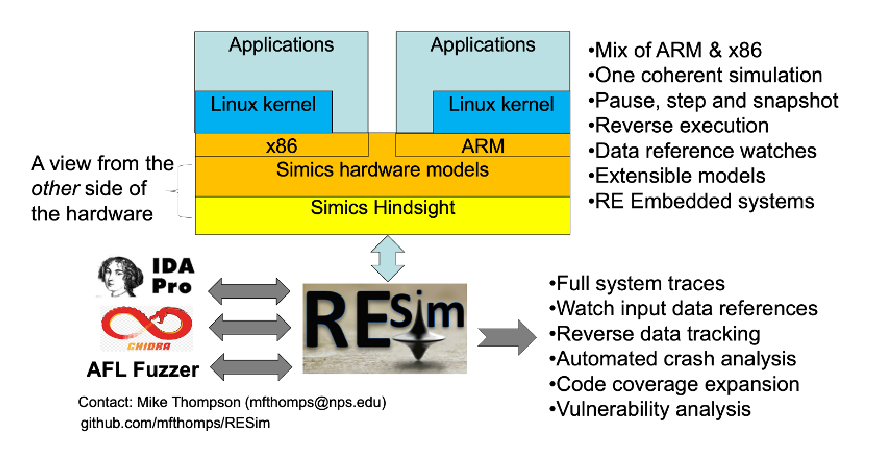
\includegraphics{resimfig.eps}

\subsection{This Guide}
The remainer of this introduction provides an overview of RESim features and its limitations and availability.  Following the introduction:
\begin{itemize}
\item Section \ref{workflow} 
describes a notional workflow, highlighting functions and features of RESim and how an analyst might use them to reverse engineer a 
network of computers.  
\item The set of commands supported by RESim are listed in section \ref{commands}.  
\item Section \ref{configuration} details
the elements of RESim configuration files (ini files) that define the system to be simulated.  
\item The mechanics of installing and running 
RESim are described in section \ref{running}.  This includes descriptions of data tracking (forward and reverse) and code coverage. 
\item Example workflows for RESim are provided in section \ref{example-workflows}.  
\item Example disk images and targets are listed in section \ref{example-targets}.
\item Use of AFL to expand code coverage and identify vulnerabilities is described in section \ref{fuzz}.
\item Section \ref{implementation} describes the implementation strategy and some of its consequences.
\item Section \ref{troubleshooting} provides some trouble-shooting tips.
\item The Appendices provide a set of notes and hints that have not yet been integrated into the body of the guide.
\end{itemize}

\subsection{Analysis artifacts}
RESim generates system traces of all processes on a computer, starting with system boot, or from a selected checkpoint.  Trace reports include two components: 
\begin{enumerate}
\item A record of system calls, identifying the calling process and selected parameters, e.g., names of files and sockets and IP addresses.
\item A process family history for each process and thread that has executed, identifying:
\begin{enumerate}
\item Providence, i.e., which process created the process (or thread), and what programs were loaded via the {\tt execve} system call.
\item Files and pipes that had been opened (including file descriptors inherited from the parent), and those that are currently open.
\item Linux socket functions, e.g. , connect, accept, bind, etc.  Socket connect attempts to external components are highlighted, as are 
externally visible socket accepts.
\item Mapped memory shared between processes
\end{enumerate}
\end{enumerate}

The system trace is intended to help an analyst identify programs that consume externally shaped data.  Such programs can then be analyzed in depth with the dynamic disassembler. [TBD expand to support decompilers where available].  

Artifacts associated with individual processes (and their associated threads) include:
\begin{itemize}
\item Maps of shared object libraries loaded by each thread, including their load addresses
\item Records of references to input data, including copies of such data, as the target program consumes the data.  These \textit{Watch Marks}, 
(see \ref{tracking}), can be dynamically loaded to skip the simulation to the point of the reference.
\item Reverse data tracks that trace sources of memory or register values in terms of exchanges between memory and registers, potentially leading
back to initial ingest of the data, e.g., via a recv system call.
\item Data written to selected files or file descriptors, (see the {\tt traceFile/traceFD} commands.
\item System traces as previously described, but constrained to actions taken by threads within the process being analyzed.
\end{itemize}

\subsection{Dynamic analysis of programs executing in their environment}
RESim couples an IDA Pro disassembler debugger client with the Simics simulation to present a dynamic view into a running process.  The analyst sets breakpoints and navigates through function calls in both the forward and reverse execution directions.  This facilitates tracking the sources of data.  For example, if a program is found to be consuming data at some location of interest, reverse execution might identify a system call that brings the data into the process’s address space.

Analysis is performed entirely through external observation of the simulated target system's memory and processor state, 
without need for shells, software injection, or kernel symbol tables.   The analysis is said to be \textit{external} because the observation functions do
not affect the state of the simulated system.  For example, when viewing code with the IDA Pro or Ghidra debugger, addresses that are not yet paged in will appear as containing zeros.
In most other systems, the debugger or its agent would run on the target, and thus the mere act of viewing the address with a debugger 
would cause the kernel to page
in the memory containing the referenced code.\footnote{See \ref{external} for another example of the implications}.

A key property that distinguishes RESim from other RE strategies is that analysis occurs on processes as they execute in their native environment, and as they interact with other processes and devices within the system.  Consider an example process that communicates with a remote computer via a network while also interacting with a local process via a pipe.  When the analyst pauses RESim for inspection, the entire system pauses.  The simulation can then be resumed (or single-stepped) from the precise state at which it was paused, without having to account for timeouts and other temporal-based discontinuities between the process of interest and its environment.

\subsection{Limitations}
RESim analyzes Linux-based systems (and some Windows based systems) for which copies of bootable media or root file systems can be obtained.  Analysis does not depend on a system map of the kernel, i.e., it works with stripped kernel images.  The current version of RESim supports 32-bit and 64-bit X86 and 32-bit ARM.  It can also be 
extended to support alternate architectures, e.g., 64-bit ARM, supported by Simics processor models \footnote{A summary of Simics device models is at: \url{https://www.windriver.com/products/simics/simics-supported-targets.html}}.  RESim is currently limited to single-processor (single core) models.  Simics supports
multi-processor simulations (at reduced performance), but RESim has not yet been extended to monitor those.
See section \ref{divergence} for information on potential divergence of simulations from real systems.

RESim and Simics are not ``record-and-replay'' tools (though Simics has that features to support that.)  We run, instrument and observe simulations of real systems.
These simulations can and will diverge from real world results and multiple runs of what seem to be the same simulation will diverge from each other (as will
multiple runs of real systems, even though they consume the same data.)  Sometimes the divergence is minimal, e.g., different timestamps within data.  Other times
the divergence can be substantial.  The point is that you should not always expect the same results across multiple runs.  For example, full system traces
may contain different data even though they commence from the same snapshot.  

\subsection{Development and Availability}
RESim is derived from the “Cyber Grand Challenge Monitor” (CGC), developed by the Naval Postgraduate School in support of the DARPA CGC competition.  
It is implemented in Python, primarily using Simics breakpoints and callbacks, and does not rely on 
Simics “OS Awareness” or Eclipse-based interfaces.   
\begin{itemize}
\item Simics is available as a commercial product from Wind River.  A free version for Intel processors is available at
\url{https://www.intel.com/content/www/us/en/developer/articles/tool/simics-simulator.html}  RESim has be exended to work with this
free versoin.

\item IDA Pro extensions are implemented using IDAPython, and are included within the RESim repo at
\url{https://github.com/mfthomps/RESim/simics/ida}  

\item The Ghidra plugins for RESim are available at: \url{https://github.com/mfthomps/RESimGhidraPlugins}  A fork 
of gdb needed for use with the Ghidra plugin is at \url{https://github.com/mfthomps/binutils-gdb}.

\item A fork of the AFL fuzzer integrated with 
RESim is available at: \url{https://github.com/mfthomps/AFL}.

\item Preliminary Windows support is provided as described in \ref{Windows.}

\item In addition to running on a local Simics installation, RESim can be offered as a network service to users running local copies of IDA Pro and an SSH session with a RESim console.  See the \textit{RESim Remote Access Guide}.  
\end{itemize}


\section{Notional Workflow}
\label{workflow}
This section provides an overview of how RESim can be used by an analyst to reverse engineer a system. Details are provided elsewhere
in this guide.  The general steps include:
\begin{itemize}
\item Extract software images from target systems.
\item Identify Simics models to simulate the target hardware.
\item Create a RESim workspace directory with which to run the simulation
\item Construct a RESim configuration file to identify system image file locations and RESim parameters.
\item Use RESim to extract a set of kernel parameters if not already extracted for the kernel images being used.
\item Run the simulation to produce full system traces and processing reports for the simulated systems.
\item Identify processes of interest, and use the RESim IDA Pro debugging client to analyze their behavior, e.g, the protocols they consume.
\item Use the integrated AFL fuzzer to improve code coverage within the targeted process.
\item Analyze RESim sessions to identify unexplored code paths and identify input data to reach those paths, potentially feeding those back to AFL.
\item Automatically assess any crashes generated by AFL to identify potentially exploitable vulnerabilities.
\item Use RESim to analyzing the vulnerabilities and craft proof of concept exploits.
\end{itemize}

\subsection{Workspace directories}
Simics simulations are run from workspace directories prepared using the {\tt resim-ws.sh} command, which creates a Simics workspace within a new empty
directory and populates it with selected RESim files.  The workspace is where simulation-specific configuration files and scripts are to reside.  Snapshot
data is also stored within workspace directories.  You may share snapshots between workspaces by using symbolic links.  

\subsection{Configuration files}
Simulated systems are defined within RESim configuration files (see \ref{configuration} that  parameterize pre-defined Simics scripts to identify 
processors and interface devices, e.g., network cards, disks and system consoles.  RESim currently includes the following platforms: 
\begin{itemize}
\item A general purpose X86 platform with disk, multiple ethernet and serial ports;
\item A generic ARM Cortex A9 platform with disk, multiple ethernet and serial ports.
\item An ARMV5 platform based on the ARM926EJ-S processor.  This is a partial implementation of the ARM Integrator-CP board.  It currently only supports
the initial RAM disk, one ethernet and serial ports.
\end{itemize}

Other platforms can be modeled via Simics, the detailes of which are beyond the scope of this manual.
Once a system is modeled and referenced by a RESim configuration file, a RESim script is run, naming the configuration file.

\subsection{Kernel parameter extraction}
RESim analysis requires about twenty parameters that characterize the booted kernel instance, e.g., offsets within task 
records and addresses of selected kernel symbols.  The CREATE\_RESIM\_PARAMS directive within the RESim configuration file directs the tool to automatically analyze the running kernel 
and extract the desired parameters.  This allows RESim to analyze disparate Linux kernels without a priori 
knowledge of their versions or configurations \footnote{Not to be confused with the similar function included with Simics Analyzer product. RESim uses an alternate strategy for OS-Awareness.}.
See section \ref{getting-started}.

\subsection{Find interesting processes}
Once the kernel parameters have been extracted, the RESim configuration file is modified to reference the parameter file, and the simulation is restarted. The user is
presented with a command line interface console.  This console manages the simulation via a combination of RESim and Simics commands, including commands to:
\begin{itemize}
\item Start or stop (pause) the simulation
\item Run until a specified process is scheduled
\item Run until a specified program is loaded, i.e., via execve
\item Generate a system trace
\item Inspect memory and component states
\item Enable reverse execution, i.e., allow reversing to events from that point forward
\item Set and run to breakpoints, either in the future or in the past.
\item Target RESim to focus on a specific process thread group, e.g., for dynamic analysis using IDA Pro.
\end{itemize}
\noindent See section \ref{commands} for details of RESim commands.

A typical strategy with RESim is to initially perform a full system trace on a system as a means of identifying programs of interest, e.g., which can then be
further analyzed using the interactive IDA Pro client.  The {\tt traceAll} command described below in \ref{commands} generates such a trace.  Note that a typical Linux-based
system can perform tens of thousands of system calls during initial boot processing.  It may save considerable time to use the {\tt toProc} command to run forward to some
event such as creation of {\tt rsyslogd} before issuing the {\tt traceAll} command.  Note that {\tt toProc} tracks processes creation and some system configuration settings such as
IP addresses set using {\tt ip} or {\tt ifconfig} commands, which can be seen using the {\tt showNets} command.  Use the {\tt writeConfig} command to create a checkpoint,
and then update your ini file to begin at that checkpoint using the {\tt RUN\_FROM\_SNAP} directive.  Trace files are created in the ./logs directory.  During a trace, if you use the Simics stop and
run commands, the tracing will continue.  While stopped, you may use the {\tt tasks} commands to see which processes are currently running.  Or the {\tt showBinders} command to 
see network ports being listened to. See the \ref{process_tracing} for more information about process tracing. 

\subsection{Analyze a process}
When RESim is targeted for a given process it runs until that process is scheduled, after which the user starts IDA Pro with a suite of custom plugins that interact with the simulation.  If a binary image of the target program is available, standard IDA Pro analysis functions are performed.  If no program image is available, IDA Pro will still present disassembly information for the program as it exists in simulated system memory.  

RESim extends IDA Pro debugger functions and the analyst accesses these functions via menus and hot keys.   The disassembler/debug client can be used to:
\begin{itemize}
\item Single-step through the program in either the forward or reverse direction
\item Set and run to breakpoints in either direction
\item Run to the next (or previous) system call of a specified type, e.g., open.
\item Run to system calls with qualifying parameters, e.g., run until a socket connect address matches a given regular expression.
\item Track references to data read in via a given FD, as well as refererences to copies of that data, e.g., via {\tt memcpy}.
\item Reverse-trace the source of data at a memory address or register.
\item Modify a register or memory content
\item Switch threads of a multithreaded application
\item Set and jump to bookmarks
\end{itemize}

\subsection{Code coverage with AFL}
Using RESim to understand the protocols handled by a process, (and associated vulnerabilities),  typically involves providing the process with
crafted data and observing its behavior and modifying data to achieve greater code coverage.  AFL contributes to code coverage expansion
and vulnerability identification through automated guided fuzzing.  AFL provide RESim with randomized inputs that 
it continually augments based on feedback that RESim generates reflecting code paths reached by each input.  

A set of RESim functions can then be used to replay AFL sessions to automatically identify and display unexplored code paths within
the IDA client.  This allows the analyst to identify and generate inputs for additional code paths, and feed these inputs back into 
new AFL sessions.  See section \ref{fuzz} for information on the use of AFL.

See \ref{example-workflows} for detailed examples of RESim workflows.


\section{RESim commands}
\label{commands}
The following RESim commands are issued at the Simics command prompt, naming the commands as methods of the {\tt cgc} python module,
e.g., "{\tt @cgc.tasks()}".  Interfaces for all of these commands are implemented in the python script at {\tt simics/monitorCore/genMonitor.py}
If this documentation falls out of sync, or you need to fix broken stuff, refer to that file (and the dependent python classes, which are all in that directory.)

There are also a set of utility commands that run from a bash prompt (rather than from Simics).  See section \ref{utilities} for a list of those.

\label{commands}
\subsection{General display}
\begin{itemize}
\item {\tt show} -- Show current process information for the currently monitored target.
\item {\tt tasks(filter=None)} -- List currently executing process names and their PIDs for the currently monitored target. Use a simple string filter to view information on
a specific program.
\item {\tt showThreads} -- List threads of process currently selected for analysis, e.g., via {\tt debugProc}.
\item {\tt showTargets} - List the target cells that may be monitored.
\item {\tt setTarget} -- Set the currently monitored target.
\end{itemize}

\subsection{Process tracing}
\label{process_tracing}
The tracing commands described below are applied to the currently selected target system.  If you wish to trace multiple simulated computers, select
each using {\tt setTarget} and issue the {\tt traceAll} command.  Note traces are not necessarily repeatable, i.e., there is usually execution 
divergence between different runs, even when starting at the same snapshot.  Trace artifacts are written to the logs subdirectory of the workspace.

Within a given simulated computer the scope of which processes are traced has four forms:
\begin{enumerate}
\item All processes are traced as they are scheduled and run.
\item When debugging a selected program, only the threads within the associated process are traced.
\item If {\tt ONLY\_PROGS} is set in the ini file, then only the programs listed in the named file are traced.
\item If {\tt SKIP\_PROGS} is set in the ini file, then all programs other than those listed in the named file are traced.
\end{enumerate}

A common use of process tracing is to create artifacts describing network usage, e.g., which ports are bound by which processes.  Note that RESim tracks
such things by watching system calls.  Thus, if you only start tracing a process \textit{after} it has bound to a port, then RESim will not tell you that
the process is bound to the port.

When tracing is selected, RESim will track loading of shared program libraries.

\begin{itemize}
\item {\tt traceAll} – Begin tracing all system calls, storing the results in the logs subdirectory of the workspace.  
If a program was selected using debugProc as described below, limit the reporting to that process and its threads.  
To limit tracing to the current thread, first issue the {\tt debugThis} command.
See the {\tt saveTraces} command below, and the {\tt traceReport.sh} script which will parse system call logs and create reports on file, network and IPC (System V) usage.
\item {\tt traceProcesses} – Begin tracing the following system calls as they occur:
vfork; clone; execve;  open; pipe; pipe2; close; dup; dup2; socketcall; exit; group\_exit
Tracing continues until the stopTrace command is issued.  
\textbf{Note} Generally use traceAll instead of this command.  This command has some value in that it results in breakpoints on calculated entry points vs
sysenter type entry points.  This may aid in some RESim debugging.

\item {\tt saveTraces} -- Combines the next 4 items and saves the results in the workspace/logs directory.  This is typically done after doing a traceAll
on either an entire component, or a program.  After running {\tt saveTraces}, exit Simics, cd to the logs directory and run {\tt traceReport.sh} to parse
the trace artifacts and create summaries, e.g., a summary of all services accessing networks.
\begin{itemize}
\item {\tt showProcTrace} – Generate a process family summary of all processes that executed since the traceProcess (or traceAll) command.

\item {\tt showNets} – Display network configuration commands (e.g., {\tt ifconfig} collected from process tracing and the use of toProc.

\item {\tt showBinders} – Display programs that use bind and accept socket calls – intended for use during process tracing to identify processes that listen on externally accessible sockets.

\item {\tt showConnectors} – Display programs that use connect to open sockets – intended for use during process tracing to identify processes that connect to externally accessible sockets.
\end{itemize}

\item {\tt traceFile(logname)} – Copy all writes that occur to the given filename.  Intended for use with log files.  Output is in ./logs/[basename(logname)].
The {\tt trackIO} command can be directed to include traced file output in the watch marks, e.g., to see where log messages occur within the
time line of watch marks.

\item {\tt traceFD(FD)} – Copy all writes that occur to a given FD, e.g., stdout.  Output is in ./logs/output-fd-[FD].log   Assumes traceAll is set.

\item {\tt buffer tracing} – Use the {\tt TRACE\_BUFFERS} environment variable to report on use of debug buffers.  Syntax of each line is:
\begin{verbatim}
   call_reg  <addr> <reg> <outfile>
\end{verbatim}
Where \textit{addr} is the address of an instruction, typically a call to some some sprintf function within a debug routine, \textit{reg} names the register that containing the address of the debug message
and \textit{outfile} is the name of the file into which the messages should be written.

\item {\tt flushTrace} - Flush trace output to the trace log files.

\item {\tt toProc} – Continue execution until the named program is either loaded via execve or scheduled.  Intended for use prior to tracing processes, e.g., to get to some known point before incurring overhead associated with tracing.   This function will track processes PIDs and names along with network configuration information, and will save that data if a writeConfig function is used.
Use an optional {\tt run=False} to prevent RESim from continuing the simulation, e.g., so that you can run commands such as ptime.

\item {\tt autoMaze} -- Avoid being prompted when tracing detects a crude timing loop or other events that are repeated many times in a loop.
See section \ref{maze}.

\item {\tt instructTrace(file, all\_proc=False, kernel=False, watch\_threads=False) -- Generate an instruction trace and save it into the named file. Use the kernel
flag to observe traces within the kernel. Use {\tt watch\_threads} to trace all threads of the current process.}
\end{itemize}

\subsection{Saving state}
A \textit{snapshot} of the system state can be created at any time and then named within the ini file using the {\tt RUN\_FROM\_SNAP} environment variable.

\begin{itemize}
\item {\tt writeConfig} – Uses the Simics write-configuration command to save the simulation state for later loading with read-configuration.  This wrapper also saves process naming information, shared library object maps and network configuration commands for reference subsequent to use of the read-configuration function.
\item Also see prepInject.
\end{itemize}

\subsection{Shared libraries}
RESim tracks loading of shared libraries within processes depending on the current scope of tracing or whether the program
is being debugged.
If a program is to be analyzed, then it is critical that the program's use of shared libraries be tracked.  When system state is 
saved to a snapshot, the shared library information is saved and then restored when the snapshot is loaded.

When {\tt traceAll} is used, all traced processes will have their shared libraries tracked.  If a process is being debugged, e.g.,
through use of {\tt debugProc}, then its shared library loading will be tracked both as it loads, and then as it is run forward.
If processes of interest are not being traced or debugged, then then {\tt trackThreads} command will cause library loading to be tracked.

\begin{itemize}
\item {\tt trackThreads} Causes RESim to track shared library loading for all processes on the selected target, filtered by either the
{\tt ONLY\_PROGS} or {\tt SKIP\_PROGS} directives in the ini file.
\item Use of {\tt traceAll} or {\tt traceWindows} will cause tracking of libraries.
\item {\tt showSOMap(filter=None)} will display the SO map of the current process.  Use the filter to select based on string content.
\item {\tt getSO(addr, show\_orig=False)} Display the shared library file and and address range within which the given address falls.
If the {\tt show\_orig} option is given, then the original program base address is displayed as well.
\end{itemize}

\subsection{Process Analysis}
These functions support interactive analysis of the threads of a process, e.g., to run until some system call is made.  Also see the \textit{Tracking data} functions
in the following subsection.  Analysis functions depend on shared library data gathered while the target process is being loaded and initialized.  In general, you
must use the {\tt debugProc} function to capture that information.  You may then create a checkpoint.  Subsequent sessions started from that checkpoint,
or subsequent checkpoints, can then use alternate functions to select debugging, e.g., the {\tt debugPidGroup} function. RESim gathers shared library information on
all processes started while processing the {\tt debugProc} command, so it is possible to create checkpoints from which multiple processes can be selectively
debugged.  To put this another way, you cannot choose to debug some process that is already running on the simulated system unless you took steps to
gather its shared library data prior to the process being loaded.

\begin{itemize}

\item {\tt debugProc(process name)} – Initiate the debugger server for the given process name.  If a process matching the given name is executing, system state advances until the process is scheduled.  If no matching process is currently executing, execution proceeds until an execve for a matching process.   If a copy of the named program is found on the RESim host, (i.e., to read its ELF header), then execution continues until the text segment is reached.  RESim tracks the process as it maps shared objects into memory (see Appendix C).  The resulting map of shared object library addresses is then available to the user to facilitate switching between IDA Pro analysis and debugging of shared libraries and the originally loaded program.

The process name is searched against the comm names, which are fifteen characters.  RESim will trucate input names to 15 characters.
                                                               

Subsequent to the debugProc  function completion, IDA Pro can be attached to the simulator.  Most of the commands listed below have analogs available from within IDA Pro, once the RESim {\tt rev.py} plugin is loaded.

If execution transfers to a shared object library of interest, the associated library file can be found via the origProgAddr command described below.  Load that file into IDA Pro and rebase to the SO address
found via showSOMap prior to attaching the debugger.  If you have run reTrack or injectIO, you must re-run the command in order for the Watch Marks to 
detect and report mem operations, e.g., memcpy -- and then refresh the IDA Data Watch window. 

If you prefix the given process name with {\tt sh }, (sh followed by a space), RESim will look for a shell invocation of the script name that follows the sh.

\item {\tt debugTidGroup(tid)} -- Initiate the debugger server for a given TID.  Intended for use after starting a session from a checkpoint created using
{\tt writeConfig}.  This assumes process information had been generated in a previous session that was saved.  

\item {\tt debugSnap} -- Assumes the current session was loaded from a snapshot, it use debugPidGroup to debug the process being debugged when the snapshot was made.
\textbf{NOTE} If you use debugSnap after running for a while, you may well lose process state, specifically system call information about 
threads that are waiting in the kernel.  If you want to run ahead to let the system settle out, first use debugSnap and then use noReverse to improve speed.

\item {\tt debugIfNot} -- Will call debugPidGroup for the currently scheduled process.

\item {\tt debugThis} -- Limit debugging to the current thread, ignoring other threads.

\item {\tt getStackTrace} – shows the call stack as seen by the monitor.  The Ida client uses this to maintain its view of the callstack.  The monitor
uses the IDA-generated function database ({\tt .fun} files stored wtih the {\tt .idb} files to aid in determining if 
potential instruction calls are to functions.  The monitor-local {\tt stackTrace} command displays a
stack trace that uses the IDA function database to resolve names.  (TBD, does not yet handle plt, and thus shows call addresses for such calls).
This function is not always reliable, e.g., phantom frames may appear based on calls that occurred previously. ARM stack frames may be
difficult to determine due to its myriad ways of calling and returning. 

\item {\tt runToSyscall(call number)} – Continue execution until the specified system call is invoked.  If a value of minus 1 is given, then any system call will stop execution.  The simulation stops after the return from the call.  If the debugger is active, then the simulation only halts when the debugged process makes the named call.

\item {\tt runToCall(call name)} – Continue execution until the specified system call is invoked.  The simulation stops at the system call kernel entry.
If the debugger is active, then execution only halts when the debugged process makes the named call.

\item {\tt revToSyscall()} -- Reverse to previous syscall made by the current process.

\item {\tt runToConnect(search pattern)} – Continue execution until a socket connection to an address matching the given search pattern.

\item {\tt runToBind(search pattern)} – Continue execution until a socket bind to an address matching the given search pattern.  Alternately, providing just
a port number will be translated to the pattern {\tt .*:N\$} where N is the port number.

\item {\tt runToAccept(FD)} – Continue execution until a return from a socket accept to the given file descriptor.

\item {\tt runToIO(fd, nth=1)} – Continue execution until a read, write, select, ioctl, accept or close with the given file descriptor.  
If nth is greater than 1, will run until the nth recv call.  

\item {\tt runToInput(fd)} -- Like runToIO, but only finds reads, receives, etc.

\item {\tt runToOpen(file)} -- Stops at the open of a given filename.

\item {\tt runToWrite(substring)} -- Stops when a process writes the given substring via a system call.

\item {\tt clone(nth)} – Continue execution until the nth clone system call in the current process occurs, and then halt execution within the child.

\item {\tt runToText()} – Continue execution until the text segment of the currently debugged process is reached.  DO NOT use for Windows.  Use runToSO instead. 
This, and revToText, are useful after execution transfers to libraries, or Linux linkage functions, e.g., references to the GOT.

\item {\tt revToText()} – Reverse execute the current process until the text segment is reached.  Also useful when you get lucky and execution is down a nop sled.  This function can be slow, e.g., if there is a kernel system call between you and the text segment.
 
\item {\tt showSOMap(tid, filter=none)} – Display the map of shared object library files to their load addresses for the given pid (along with the main text segment).
Use a simple string filter to look for a particular library.

\item {\tt origProgAddr(pid, addr)} – Display the program file name (e.g., library) and load address of the shared object containing the given address.  Also displays the 
original program address, e.g., to include a jumper file for use over multiple load instances.

\item {\tt revInto} – Reverse execution to the previous instruction in user space within the debugged process. 

\item {\tt revOver} – Reverse execution to the previous instruction in the debugged process – without entering functions, e.g., any function that may have returned to the current EIP.  Note that ROP may throw this off, causing you to land at the earliest recorded bookmark.  Use {\tt revInto} to reverse following a ROP.

\item {\tt uncall} – Reverse execution until the call instruction that entered the current function.  This may be unreliable with some ARM
programs.

\item {\tt revToWrite(address)} – Reverse execution until a write operation to the given address within the debugged process.

\item {\tt revToModReg(reg)} – Reverse execution until the given register is modified.


\item {\tt toPid(pid)} -- Run forward until the given pid is scheduled.  Use {\tt -1} to indicate any of the threads being debugged.

\item {\tt runToUser()} – Continue execution until user space of the current process is reached.

\item {\tt reverseToUser()} – Reverse execution until user space of the current process is reached.

\item {\tt setDebugBookmark(mark)} – set a bookmark with the given name.

\item {\tt goToDebugBookmark} – jump to the given bookmark, restoring execution state to that which existed when the bookmark was set.  The
{\tt listBookmarks} command will list bookmarks, displaying  index numbers.  These numbers can be provided to the {\tt goToDebugBookmark} command instead
of the bookmark string.  Note these bookmarks are separate from the data watch bookmarks, which can be viewed using the {\tt showWatchMarks} command.

\item {\tt runToKnown} Continue execution until a text range known to the SOMap (see {\tt showSOMap()}).  Intended for use if execution stops in got/plt 
or other loader goo.

\item {\tt runToOther} Continue execution until a text range known to the SOMap (see {\tt showSOMap()}) -- but not the current text range -- is entered.
Useful if you are in some library called by some other library, and you want to return to the latter.

\item {\tt runToSO} Continue execution until a given program, SO or DLL file is reached.

\item {\tt doBreak} Sets a breakpoint on a given address.  This command can be useful when wishing to break while running other commands.  For example,
using {\tt doBreak} prior to running {\tt injectIO} may be more reliable than simply setting a Simics break and it will clean up other breaks and haps that 
might interfere with your subsequent analysis.

\item {\tt runToWriteNotZero(addr)} – Run forward until a non-zero value is written to the given memory address.


\end{itemize}

\subsection{Data tracking}
Also see \ref{tracking}
\begin{itemize}

\item {\tt trackIO(FD, reset=False, count=1, mark\_logs=False, kbuf=False, run=True, commence=None)} -- Combines the {\tt runToIO} and the {\tt watchData} functions to generate a list of data watch bookmarks that indicate execution
points of relevant IO and references to received data.  This list of data watch bookmarks is displayed using {\tt showWatchMarks} or in the IDA client {\tt data watch} window (right click and refresh).
If an {\tt accept} call with the given FD is detected, the FD being tracked will be changed to that returned by the accept call.
The trackIO function will break simulation after {\tt BACK\_STOP\_CYCLES} with no data references. If the debugged processes are in the kernel waiting to read on the given
FD, RESim will ensure that call is tracked.  The count parameter can be used to track the Nth read or recv.   Data watches persist after the
call, e.g., to support {\tt retrack} described below.  Each use of trackIO will reset all data watches, but does not clear watch marks, i.e., you can still skip to those simulation cycles.  Also see 
the {\tt tagIterator} command.  The {\tt reset} parameter will cause the reverse time origin to be reset if the kernel was waiting on a read/recv. See \ref{real-networks}  Data to be consumed by the taget can originate from a simulated computer, e.g., a driver, or via a real network using something like:
\begin{verbatim}
    cat foo.io > /dev/udp/127.0.0.1/6060 
\end{verbatim}
\noindent Note that sending multiple packets via real networks will cause the origin to reset on each packet, thereby limiting the range of reverse execution.  It is generally simpler
to use a driver computer to send multiple packets, using a program such as {\tt simics/bin/drive-driver.py}.  The {\tt -d} option of that program executes the Simics magic instruction to cause RESim to reset
its origin just prior to the initial data transmission.  This also causes RESim to disconnect the real network to ensure that the reversible range does not receive any real-word leakage.

Use of the {\tt mark\_logs} option will include corresponding log entries from any use of {\tt traceFile} as watch marks.  This may help display diagnostics
within your watch mark list as parsing encounters errors.

The {\tt kbuf} option is used in conjunction with prepInjectWatch to record kernel buffers used when receiving the data.  This data must be populated with 
a designated character, currently ``Z''.  And there must be as much data as you expect to read during injectIO sessions.  The designated characters are used by
RESim to identify the end of individual kernel buffers, and thus are critical to determining the size and location of the different kernel buffers.  It is also
critical that the data be of a form that will be read by the application because RESim locates kernel buffers by backtracing data read into application buffers.
However, if you find the first kernel buffer is as large as any data you might send, then a single application read will suffice.
If AFL filters are to be used, e.g., to generate CRCs, then apply the filter before sending the data to the target via the driver.
Take care to avoid extranious characters, e.g., newlines at the end of the test data.

Use an optional {\tt run=False} to prevent RESim from continuing the simulation, e.g., so that you can run commands such as ptime.

Use an optional {\tt commence=string} to delay data tracking until the received data starts with a given string.  This can be useful when a socket receives a lot of traffic and you
wish to focus on traffic that you are sending.

\item {\tt trackProgArgs} Track references to arguments provided to the program as argv values.

\item {\tt trackCGIArgs} Track references to arguments provided to the program as packaged by cgi-bin.

\item {\tt retrack} -- Intended for use after modifying content of an input buffer in memory.  This will track accesses to the input buffer.
Note that this function does record additional IO operations, BUT WILL reflect subsequent access to the existing watch buffers.  (TBD, terminate on access
to remembered FD?)

\item {\tt trackFile} -- Currently works only with files opened by xmlParseFile. The function notes all memory malloc'd within
xmlParseFile and then tracks its access, e.g., via xmlGetParam, adding watch marks as it goes.

\item {\tt showWatchMarks(old=False)} Display a list of watch marks created by watchData or trackIO.  Use the {\tt old} flag to view stale watch marks, i.e., 
those that occurred prior to the origin (which gets reset on each data injection.)

\item {\tt goToDataMark(watch\_mark)}  Skip to the simulation cycle associated with the given {\tt watch\_mark}, which is an index into the list of data watch bookmarks generated by {\tt trackIO} or {\tt injectIO}.

\item {\tt getWatchMarks()} Return a json list of watch marks created by watchData or trackIO, used by the IDA client.

\item {\tt tagIterator(index)} Tag a watch mark as being an iterator.  The associated function is added to a file stored along with IDA functions
The intent is to avoid data watch events on each move, or access, e.g., a crc generator.

\item {\tt trackFunctionWrite(fun)} Record all write operations that occur between entry and return from the named function.

\item {\tt goToWriteMark(write\_mark} Skip to the simulation cycle associated with the given {\tt write\_mark}, which is an index into the list of 
write watch bookmarks generated by {\tt trackFunctionWrite}.

\item {\tt getWriteMarks()} return a json list of write marks created by {\tt trackFunctionWrite}.

\item {\tt revTaintReg(reg)} – Back trace the source of the content the given register until either a system call, or a non-trivial computation (for evolving definitions of “non-trivial”.  

\item {\tt revTaintAddr(addr)} -- Back trace the source of the content the given address until either a system call, or a non-trivial computation

\item {\tt injectIO(iofile, stay=False, n=1, target=None, targetFD=None, cover=False, break\_on=None, trace\_all=False, mark\_logs=False, no\_reset=False)} -- Assumes you have previously used {\tt prepInject}
to create a snapshot (see \ref{prepInject} and that snapshot has been loaded.
The content of the given {\tt iofile} is written into the read buffer, and the register reflecting 
the count is modified to reflect the size of the file.  If {\tt stay} is False, the {\tt retrack} function is then invoked. If {\tt keep\_size} is
set, then the size register will not be altered, which is intended for use when replaying files trimmed by AFL.
This injectIO function intended use is to rapidly observe execution paths for variations in input data. The command will automatically
run the debugPidGroup command on the current TID. The optional {\tt n} parameter causes the data file to be treated as n different packets.
The optional {\tt target} and {\tt targetFD} parameters name a different process and its FD whose data references are to be tracked.  For example,
if the original receiving process does some processing and sends derivative data to a pipe, the target could be the process at the read side
of the pipe.  If the {\tt cover} parameter is true, code coverage will be tracked and saved in a hits file.  This may take a while -- wait for the
Simics prompt to display a message such as {\tt Coverage saveCoverage to...}.

The break\_on will break on execution of the given address. 

The trace\_all option will generate a system call trace instead of watch marks.

Use mark\_logs to include log entries generated using traceFile or traceFD within the watch marks.

Use no\_reset to stop the simulation rather than resetting the origin, e.g., to adjust a return value from a read.

\item {\tt traceInject(iofile)} -- (DEPRECATED) See the {\tt trace\_all} options to injectIO and playAFL.

\item{\tt traceMalloc} -- track calls to the malloc and free functions and includes those events in the list of watch marks. Use {\tt showMalloc} to 
then list by pid, block address and size.

\item {\tt watchData} – run forward until a specified memory area is read.  Intended for use in finding references to data consumed via a read system call.  Data watch parameters are automatically set on a read during a debug session, allowing the analyst to simply invoke the watchData function to find references to the buffer.  List data watches using {\tt showDataWatch}.
Note however, that data watches are based on the len field given in the read or recv, and thus data references are not necessarily to data actually read (e.g., a read of ten bytes
that returns one byte would break on a reference to the fifth byte in the buffer.)

\end{itemize}

\subsection{Vulnerability detection}
\begin{itemize}
\item {\tt catchCorruption} – Watch for events symptomatic of memory corruption errors, e.g., SEGV or SIGILL exceptions resulting from buffer overflows.  This is automatically enabled during debug sessions. Refer to \ref{SEGV} for information about what we mean by SEGV, and how we catch it.

\item {\tt watchROP} -- Watch for return instructions that do not seem to follow calls.  This is available while debugging a process.
\end{itemize}

\subsection{System modification}
\label{sec:modification}
\begin{itemize}

\item {\tt writeReg} – Write value to a register (Note: deletes existing bookmarks.)
\item {\tt writeWord} – Write word to an address. This function will delete existing bookmarks and craete a new origin.  If there are data watch marks,
i.e., from a trackIO, these are deleted except for any that are equal to the current cycle.  The upshot of this is that if you want to modify memory
and then rerun a trackIO, do so while at the first datamark.
\item {\tt writeString} - Write a string to an addrss. Use double escapes, e.g., two backslashes and an n for a newline. (Note: deletes existing bookmarks.)

\item {\tt runToDmod(dmod\_file)} – Run until a specified read or write system call is encountered, and modify system memory such
that the result of the read or write is augmented by a named Dmod directive file.  See \ref{dmod}

\item {\tt readReplace(readrelace\_file)} – Replace memory content with a given hex string when that memory address if first read by the program.

\item {\tt modFunction(fun, offset, word)} Write the given word at an offset from the start of the named function.  Intended for use in setting return
values, e.g., force eax to zero upon return.  Bring your own machine code.  TBD accept an assembly statement?

\item {\tt showLinks} - Display symbolic names of network connections.  These may then be used in DMOD directives, or manually using Simics {\tt connect}
and {\tt disconnect} commands.

\item {\tt jumper(from, to} - Alter control flow by causing execution to jump to a given address whenever a given {\tt from} address is hit.  See
the {\tt EXECUTION\_JUMPERS} ini environment value.

\end{itemize}
\subsection{Code coverage}
\begin{itemize}
\item {\tt mapCoverage} -- Set breakpoints on all basic blocks in the text segment and use them to track code coverage. The basic block coverage is
saved in a $<$prog$>$.hits file in IDA db directory, and will be read by the IDA client when the {\tt color} option is used. Subsequent uses of {\tt mapCoverage}
will reset the coverage tracking.  Use {\tt stopCoverage} to stop basic block tracking.  The basic blocks database is read from the .blocks file created
by the IDA client findBlocks script.  See section \ref{coverage} for information on how the IDA client represents code coverage and highlights
branches that have not been taken.

\item {\tt showCoverage} -- display summary of basic block coverage.  Also see the IDA client {\tt color} and {\tt clear} options.

\item{\tt goToBasicBlock} -- Skip the simulation state to the first hit of the block named by an address (requires use of {\tt mapCoverage}..

\item{\tt addJumper(from, to)} -- Define a jumper to cause execution to skip from a from block to a to block.  These are intended for use with code coverage and fuzzing (see \ref{jumpers}).
Use {\tt jumper(from, to)} for general execution jumpers.
\end{itemize}

\subsection{Fuzzing}
\begin{itemize}

\item{\tt afl(fname=None, target=None, targetFD=None, dead=False)} -- Typically the {\tt runAFL} utility (from a bash shell in your workspace directory) is used instead of this command.  Uses a network connection to communicate AFL server \url{github.com/mfthomps/AFL}.  
The simulation is assumed to loaded from a checkpoint created using {\tt prepInject}.  Provide {\tt fname} to name a library, i.e., if the program's main
text blocks is not what is to be instrumented.
Use {\\tt target} and {\tt targetFD} to name some other process 
and the FD from which it reads if the fuzzing target is other
than the consumer of the AFL-generated data.  The {\tt dead} option creates a filter to avoid instrumenting basic blocks hit by other threads.
Use {\tt aflTCP} for TCP sessions, though note these assume all data is read into
the same input buffer.  
See section \ref{fuzz} for details.

\item{\tt prepInject(fd, configfile, count=1, commence=string)} -- Prepares a simulation for injectIO or fuzzing by running to an input system call for the given FD.  It saves the post-call state in a snapshot
file with the given name.  Saved state includes the syscall call and return instruction addresses for use in multi-packet UDP fuzzing, and buffer address and size.
Note using this with TCP and real networks can lead to undefined behavior, and thus you should use a driver computer instead of real networks.  
Use the count to stop the simuation subsequent to the nth input system call, e.g., to get an initial state for fuzzing that is predicated on a preamble exchange.
This may require use of the {\tt simics-magic} program on a driver computer.  See \ref{prepInject} for details.

Note that the data you provide for prepInject should not include multiple UDP packets because you want the recv to not see more data after consuming your
subsequent data injections.

Consider providing prepInject with largish amounts of data to ensure buffers that may cross page boundaries are populated.

Use the {\tt commence=string} option to ignore input that does not start with the given string.  

\item{\tt prepInjectWatch(watchmark, configfile)} -- For use when preparing to inject data directly into kernel buffers.  
Similar to prepInject but takes the index of a watch 
mark that can be a call to ioctl, or a call to read/recieve. Generate the data marks by using trackIO, and providing the maximum amount of data you expect to 
read from kernel buffers.
Use of the resulting snapshot with AFL or injectIO will cause the data to be injected
into a kernel buffer. If the watch mark was an ioctl call, the kernel's buffer pointer values will be adjusted to reflect the new data size.  Note this command does not support running forward past the application
references to the input data, e.g., the kernel may detect corruption on the recv following the end of the current data.
Do not try to run these checkpoints forward to establish new checkpoints.
It is important that received data all appears within the kernel buffer before the application is returned to from its recv call.  Otherwise, injectIO and AFL sessions
will have kernel buffers overwritten by data on the wire.  Consider using drive-driver.sh command.

\item{\tt prepInjectAddr(addr, configfile)} -- For use when preparing to inject data directly into arbitrary application memory, e.g., when fuzzing argv parameters
to a program.  Consider priming the prepInject state with enough data to cross any page boundaries that might be part of the buffer.

\item{\tt fuzz(IOFile} -- Deprecated, AFL trims data itself just fine.  Trim a data file to the minimum needed to not affect coverage. Assume the simulation is at 
a return from a read (e.g., using prepInject), set basic block coverage and iteratively execute while reducing the
IOFile data size (padding with nulls) until a minimum is found.  The final file in {\tt /tmp/trimmer} is truncated and may need to be padded to be properly consumed, e.g.,
if the program insists on reading a minimum number of bytes.  Intended for use in preparing minimal seed files for AFL.

\item{\tt playAFL(dfile, afl\_mode=False, trace\_all=False, fname=None, target=None, targetFD=None)} -- Play data input files discovered by AFL.  Assumes {\tt dfile} is a single file, or names a subdirectory of an output directory relative to the {\tt AFL\_DATA} environment variable).  
Each file in the target's {\tt queue} subdirectory(ies) will be played with code coverage tracked with new hits files generated in the {\tt RESIM\_IDS\_DATA} directory.
\textbf{Note:} While this command is running, you may see a static {\tt simics>} prompt.  That does not mean that Simics is not running -- it is an artifact of the implementation.  When running the command, you'll know it has finished when it displays where it stored the hits file.
Tail the log if you suspect it has hung.  Provide a library name as {\tt fname}, e.g., libc.so.6, to record coverage of a library.  Note if if afl\_mode is set, no hits file is generated.

If the given dfile is a file, then only that file will be played.  The {\tt afl\_mode} switch attempts to reproduce how the file was played in AFL, e.g., without temporary
breakpoints and with the AFL backstop cycles.  The {\tt trace\_all} switch will generated a system call trace.  These are intended for use in discovering why AFL
behaves in unexpected ways, e.g., lots of hangs, long sessions.

Use the {\tt target} parameter if the process whose coverage is to be tracked differs from the process into which data is to be injected.  If that occurs
on a different cell, preface the name of the target process with the cell name followed by a colon.  If you do not want to start tracking coverage
until the target has performed some number of read calls, provide the optional {\tt targetFD} and {\tt count} parameters.  For example, if you want to
commence coverage tracking after the target has returned from two read, provide a count of 2.

The {\tt playAFL} command also generates a hits file for each AFL queue file and those are stored in a {\tt coverage} directory alongside the {\tt queue} directory.
Those individual coverage files are intended to be read by the {\tt findBB.py} utility to find sessions that lead to BNTs.  Use {\tt playAFLTCP} for tcp sessions.
The {\tt runPlay} stand-alone command launches parallel instances of RESim running the playAFL, for use in replaying sessions created by parallel fuzzing.  Note however this 
does not generate a new total hits file, it only creates coverage files.  

If processes exit during replay, those will be reported after {\tt playAFL} completes replaying the sessions.

\item{\tt crashReport(dfile)} Generate crash reports for each crash discovred by AFL.  The given {\tt dfile} is as defined in the {\tt playAFL} command
NOTE: when handling multi-packet data sets, use the {\tt crashReport.py} utility (see section \ref{utilities} to launch RESim multiple times,
one for each data file.  The reports are written to /tmp/crash\_reports.

\item{\tt replayAFL(target, index, FD, [instance=N], cover=False, afl\_mode=False)} -- Replay a specific AFL session named by a target and index identifier, e.g., {\tt 0012}.  Use the optional {\tt instance} if parallel AFL is used.  This function assumes a driver component. The driver will use the sendDriver.sh script to send the named file and
a client program to the target using an address and port per the ini file {\tt TARGET\_IP} and {\tt TARGET\_PORT} values.  For UDP sessions, RESim will use the trackIO function on the given FD.  Use this to analyze multipacket processing.  For TCP, use {\tt replayAFLTCP} and the FD will be used to catch an {\tt accept} system call.  RESim will then use the returned FD for trackIO.  Set {\tt cover} to True to generate a coverage hits file.  You can then start IDA with the {\tt color} option, which
will read that hits file.   You can then double click on entries in the IDA {\tt BNT} window to skip execution to the first hit of the selected BNT source block.
Set {\tt afl\_mode} to report on blocks hit over 256 times in a session.

Note that function uses a driver to send data, and this it should not be used with a {\tt prepInject} snapshot.

\item{\tt aflInject(target, index} -- Replay an AFL session, similar to {\tt replayAFL}, except the {\tt injectIO} function is used without
a driver component.  Thus, only single-packet processing can be analyzed.  Use {\tt aflInjectTCP} for TCP sessions.

\item{\tt trackAFL(target)} -- Use injectIO to replay all AFL queue files for a given target, and store the set of resulting watch marks as json files
in the AFL output directory.  Only the first packet is tracked.  If the AFL sessions include multiple packets, then use the runTrack utlity to 
start new Simics sessions for each queue file.

\item{\tt injectToBB(bb, fname)} -- Find an AFL input file that leads to the given BB and play it using injectIO, breaking at the BB.  The target
is assumed to be the current RESim workspace directory name.  Note the simulation breaks at the BB, and thus the watch marks do not reflect subsequent
processing -- it they will not reflect any watch mark in the target BB. (TBD, modify to process/track everything, and then skip back to the first hit of the BB.)
Provide an fname if the bb is in a lib.  The bb value is per the program addresses, and RESim will adjust it to reflect the lib load address.

\item Also see utilties listed in section \ref{utilities}, e.g., to find branches not taken and AFL sessions that reach a given basic block.

\end{itemize}

\subsection{Msc}
\begin{itemize}
\item{\tt runToCycle(cycle)} -- Run to an absolute cpu cycle on the current cpu.  Useful for moving simulation forward to prepare to debug some process
that is not created until after much processing.  Cycles reported in syscall logs can help get you close to the point in time.

\item{\tt runToSeconds(seconds)} -- Run to a simulation time in seconds .  

\item{\tt satisfyCondition} -- (experimental) Assess the comparison instruction at a given address and attempt to satisfy it by altering input data.  
Initially handles simple ARM {\tt cmp reg, $<$value$>$} instructions.  The 
reverse track function is used to determine the source of the register content, and if that is a receive, it alters the data to satisfy the
comparison and then uses {\tt retrack} to run forward and track the new execution flow.

\item{\tt idaMessage} -- display the most recent message made available to IDA.  For example, after a runToBind, this will display the FD that was bound to.
\item {\tt setTarget} -- Select which simulated component to observe and affect with subsequently issued commands.  Target names are as defined in the
RESim configuration file used to start the session.

\item {\tt saveMemory(addr, size, fname)} Write a byte array of the given size read from the given addr into a file with the given name.

\item {\tt pageInfo(addr)} Use saved kernel page table addresses to get the physical address of a given linear address.  This is useful when the current
context is not that of the typical kernel state.



\end{itemize}

\section{Defining a target system}
\label{configuration}
This section assumes some familiarity with Simics.  RESim is invoked from a Simics workspace that contains a RESim configuration file.
This configuration file identifies disk images used in the simulation and defines network MAC addresses.  
The file uses {\tt ini} format and has at least two sections: and {\tt ENV} section and one section per computer that will be part
of the simulation.  An example RESim configuration file is at:
\begin{verbatim}
$RESIM/simics/workspace/mytarget.ini
\end{verbatim}
A full example target is available as described in section \ref{example-targets}.

\subsection{ENV section}
\label{env}
The following environment variables are defined in the {\tt ENV} section of the configuration file:
\begin{itemize}
\item {\tt RUN\_FROM\_SNAP} The name of a snapshot created via the {\tt @cgc.writeConfig} command.
\item {\tt RESIM\_TARGET} Name of the host that is to be the target of RESim analysis.  Currently only one host can be analyzed during a given
\item {\tt CREATE\_RESIM\_PARAMS} If set to {\tt YES}, the getKernelParams utility will be run instead of the RESim monitor.  This will
generate the Linux kernel parameters needed by RESim.  Use the {\tt @gkp.go()} command from the Simics command prompt to generate the file.
\item {\tt DRIVER\_WAIT} Causes RESim delay boot of target platforms (i.e., those other than the driver) until the 
user runs the {\tt @resim.go()} command.  Intended to allow you (or scripts)
to configure the driver platform after it boots, but before other platforms will boot.
\item {\tt BACK\_STOP\_CYCLES} Limits how far ahead a simulation will run after the last data watch event, or the last code coverage hit.
\item {\tt HANG\_CYCLES} Limits how many cycles a simulation will run under AFL until it is considered hung.
\item {\tt MONITOR} If set to NO, monitoring is not performed.
\item{\tt INIT\_SCRIPT} Simics script to be run using run-command-file.  For example, use this to attach real networks to avoid
doing so after enabling reverse execution (which should be avoided due to Simics foibles).  Do not use the name \textit{init.simics}, it seems
to confuse Simics.
\item {\tt STOP\_ON\_EXIT} Stops simulation when debugged process exits.
\item{\tt AFL\_PAD} Cause data received from AFL to be padded to this minimum packet size, intended for services having a minimum udp packet size.
This value will also be used to determine the size of writes to receive buffers when multi-packet AFL is used.
\item{\tt AFL\_UDP\_HEADER} Used with multi-packet AFL, will split data received from AFL at these strings.  If single-packet UDP sessions are desired,
leave this undefined. NOTE: initial data, e.g., AFL seeds should include the UDP header, (vice relying on filters) because the system will split input data into datagrams at the
headers \textit{prior} to applying filters.  The default maximum number of UDP packets is 10.  A maximum is needed, otherwise AFL gets carried away by duplicating
the header.  (TBD, add an env override.)
\item{\tt AFL\_PACKET\_FILTER} A packet filter to modify or weed out data received from AFL for purposes of constraining fuzzing sessions to
particualar paths, e.g., to fuzz a single command dictated by a byte at a fixed offset.  The value should be a .py file name, less the
.py extension.  The file must be relative to the Simics workspace and it must have a {\tt filter(data, packet\_num)} method that returns
the desired string.  For example, if the packet is to be rejected, return a byte array of zeros.  Filters can also be used to 
compute and store CRCs within data.  
\item {\tt AFL\_OUTPUT} -- Optional path to an AFL afl-output directory that will be referenced when running {\tt playAFL} and {\tt crashReport} commands. Typically this should not be used, and the system will use the value of {\tt AFL\_DATA} defined in the {\tt .bashrc}.
\item {\tt AFL\_MAX\_LEN} -- Maximum size of a data injection for AFL, into either kernel or user buffers. Note the trimming occurs just prior to injection,
and thus queue files and records of recent data, e.g., the ihung file, will not yet be trimmed.
\item {\tt AFL\_MAX\_PACKETS} -- Maximum size of a AFL packets written to the user space buffer.
\item {\tt AFL\_STOP\_ON\_READ} -- Stop fuzzing or tracking if the a read system call is encountered for the target FD after the fuzzed data is consumed.
\item {\tt AFL\_STOP\_ON\_CLOSE} -- Stop fuzzing or tracking if the FD is closed.  AFL queue files will be given a suffix of \textit{closed}.
\item {\tt AFL\_NO\_CALL\_HAP} -- An optimization applicable only to TCP sessions (kernel buffers) that prevents an AFL session 
from using a callHap until the buffer is consumed.  This can speed up AFL about 30 percent, depending on the application.
\item {\tt AFL\_SKIP\_READ\_N} -- Experimental... Cause every Nth read/recv to cause RESim to skip over that kernel call.  The intended use is odd
cases where a TCP session does a series of reads, then a read with a large length, but then goes back and reads a deterministic amount of data.

\item {\tt TARGET\_IP} -- IP address to use on driver fuctions such as {\tt replayAFL}
\item {\tt TARGET\_PORT} -- Port to use on driver fuctions such as {\tt replayAFL}
\item {\tt STOP\_ON\_READ} -- Cause AFL and replays to stop once the original read/recv call (or select) is hit.
\item {\tt READ\_LOOP} -- What to do if dataWatch detects a read loop, e.g., a vary large CRC calculation.  The read loop trigger defaults at 10,000
and is overridden by the {\tt READ\_LOOP\_MAX}.  A value of \textit{quit} will cause
the RESim session to exit (useful for crashReport).  Otherwise, the data watch is stopped and execution continues, e.g., to arrive at a page boundary fault.
\item {\tt READ\_LOOP\_MAX} -- Limit on dataWatch reads from a single buffer.
\item {\tt EXECUTION\_JUMPERS} -- Name of a file with jumpers (see the {\tt jumper} command in \ref{sec:modification}), expressed as 
from/to addresses in hex.  Syntax of the file is described in \ref{dynamic_control_flow}  Use \# for comments.  \textbf{Note:} encountering
a jumper will reset the reverse execution origin, and thus may not be suitable when using injectIO or crash analysis.
\item {\tt TRACE\_BUFFERS} -- Name of a file with buffer trace directives for use in capturing data written to debug buffers (regardless of whether those
buffers ever find their way to any program output). See \ref{trace_buffers}
\item {\tt RESIM\_LOG\_LEVEL} -- Set to INFO to supress debug messages in the resim log.

\end{itemize}

\subsection{Target sections}
Each computer within the simulation has its own section. The section items listed below that 
have a {\tt \$} prefix represent Simics CLI variables used within Simics scripts.  If you define your own
simics scripts (instead of using the generic scripts included with RESim), you may add arbitrary CLI variables
to this section. 
\begin{itemize}
\item {\tt \$host\_name} Name to assign to this computer.
\item {\tt \$use\_disk2} Whether a second disk is to be attached to computer.
\item {\tt \$use\_disk3} Whether a third disk is to be attached to computer.
\item {\tt \$disk\_image} Path to the boot image for the computer.
\item {\tt \$disk\_size} Size of disk\_image
\item {\tt \$disk2\_image} Path to the 2nd disk
\item {\tt \$disk2\_size} Size of 2nd disk\_image
\item {\tt \$disk3\_image} Path to the 3nd disk
\item {\tt \$disk3\_size} Size of 3nd disk\_image
\item {\tt \$mac\_address\_0} Enclose in double quotes
\item {\tt \$mac\_address\_1} Enclose in double quotes
\item {\tt \$mac\_address\_2} Enclose in double quotes
\item {\tt \$mac\_address\_3} Enclose in double quotes
\item {\tt \$eth\_device} Alternet ethernet device, see \ref{networks} below.
\item {\tt \$create\_network} Create a network service node and attach it to the named switch, intended
to provide DHCP services to targets that requrire it. See \ref{DHCP}.

\item {\tt SIMICS\_SCRIPT} Path to the Simics script file that defines the target system.  This path is relative to the {\tt target} directory
of either the workspace, or the RESim repo under {\tt simics/simicsScripts/targets}.  For example, 
\begin{verbatim}
SIMICS_SCRIPT=x86-x58-ich10/genx86.simics
\end{verbatim}
\noindent would use the generic X86 platform distributed with RESim.
\item {\tt OS\_TYPE} Either LINUX or LINUX64
RESim session.
\item {\tt RESIM\_PARAM} Name of a parameter file created by getKernParams utility.
\item {\tt RESIM\_UNISTD} Path to a Linux {\tt unistd*.h} file that will be parsed to map system call numbers to system calls.  For 64 bit
Linux, use {\tt RESIM\_DIR/linux/ia64.tbl}
\item {\tt RESIM\_ROOT\_PREFIX} Path to the root of a file system containing copies of target executables.  This is used by RESim read elf
headers of target software and to locate analysis files generated by IDA Pro. 
\item {\tt RESIM\_ROOT\_SUBDIRS} An optional semicolon separated list of subdirectories off of the {\tt RESIM\_ROOT\_PREFIX} to limit the 
search for executable images.
\item {\tt BOOT\_CHUNKS} The number of cycles to execute during boot between checks to determine if the compnent has booted enough to track
its current task pointer.  The intent is to keep this value low enough catch the system shortly after creation of the initial process.
The default value is 900,000,000, which is too large for some ARM implementations.  While components are booting, RESim uses the smallest
{\tt BOOT\_CHUNKS} value assigned to any component that has not yet completed its boot.
\item {\tt DMOD} Optional file to pass to the {\tt runToDmod} command once the component has booted.  See \ref{dmod}.
\item {\tt READ\_REPLACE} Optional file to cause memory values to be changed.  See \ref{read-replace}.
\item {\tt REG\_SET} Optional file to cause register values to be changed.  See \ref{reg-set}.
\item {\tt PLATFORM} One of the following: x86; arm; or arm5
\item {\tt INTERACT\_SCRIPT} Simics command script to be run after this component is loaded, which only occurs during boot, i.e., these are not run with snapshots.
\item {\tt ALWAYS\_SCRIPT} Simics command script to be run on each startup, reqardless of whether the run is from a snapshot.
\item {\tt ONLY\_PROGS} Optional name of a file that lists the programs that are to be watched or traced.  All others are ignored.
\item {\tt SKIP\_PROGS} Optional name of a file that lists the programs that ignored.
\end{itemize}

\subsection{Target platforms}
\label{target-platforms}
Targets platforms from the RESim {\tt simics/simicsScripts/targets} include:
\begin{itemize}
\item x86-x58-ich10 -- An x86 platform with legacy BIOS that will boot many different x86 bootable disk images. Examples can be found in
section \ref{example-targets}.
\item arm -- The Simics ARM QSP platform.  By default this boots the Simics-provided QSP kernel.  Alternately you can set the {\tt kernel\_image} 
parameter to point to a different kernel.  See the directory at:
\newline
{\tt simics/image\_build/arm-qsp} for information on rebuilding the ARM QSP kernel.  The root\_disk\_image should point to a root file system.
A stock root file system can be found at: 
\newline
\url{https://nps.box.com/v/resim-arm-qsp-rootfs}
The user\_disk|image appears as /dev/qspdc when the stock QSP kernel boots.  If it contains a partition table and file system, then the first
partition is mounted on /mnt by the stock root fs as /dev/qspdc1.

\item integrator-cp -- A 32-bit ARM platform modeled after the Integrator-cp.  A kernel and sample initrd image are at:
\newline
\url{https://nps.box.com/v/resim-arm5-images}
\end{itemize}


\subsection{Network definitions}
\label{networks}
Configuring the networks for a simulated system can require some trial and error and use of wireshark to determine which
logical eithernet devices are communicating on which simulated devices.  If you are using the predefined driver component, see the 
Appendix \ref{driver} for mappings of addresses and device names.  You may also start Wireshark from the Simics command line to 
observe which interfaces are connected to the different switches, e.g., {\tt wireshark switch0} will display traffic on switch0.
Take care to note MAC addresses and don't be fooled by packets routed through computers to other switches.

Four network switches are created, named switch0, switch1, switch2 and switch3. And two network hubs, named hub0 and hub1, are created.  
Each generic RESim computer has one or more network interfaces,
depending on the type of platform.
These are named eth0, eth1 and and eth2, and are assigned corresponding MAC addresses from the
RESim configuration file. By default, each computer ethernet interface is connected to its correspondingly numbered switch.
This topology may be modified via entries in computer sections of the RESim configuration file.  For example, an entry of:
\begin{verbatim}
ETH0_SWITCH=switch2
\end{verbatim}
\noindent would connect the eth0 deivce to switch2.  A switch value of {\tt NONE} prevents the ethernet device from being connected
to any switch.  Note there is no error checking or sanity testing.  In the above example, you would also need to re-assign the eth2 device
or it will attempt to attach two connections to the same switch port.
Alternately you can connect the ethernet devices to the hub, e.g.,:
\begin{verbatim}
ETH0_SWITCH=hub0
\end{verbatim}

Ethernet devices on the generic x86 platform default to the {\tt i82543gc} device defined by Simics.  Use of the {\tt \$eth\_dev=} 
entry lets you pick one of the following alternate ethernet devices:
\begin{verbatim}
i82559
i82546bg
i82543gc
\end{verbatim}

If using a VLAN, select the 82559.  The i82543gc does not properly support VLANs.
Note that device changes ethernet names, e.g., ens11 becomes ens11f0 and ens12 becomes ens12f0.

Simics CLI variables are assigned to each computer ethernet link using the convention {\tt \$TARGET\_eth0} where {\tt TARGET}
is the value of the configuration file section header for that component.  Similarly, connections from the computer to the switches 
are named using the convention {\tt \$TARGET\_switch0}.  These CLI variable names may be referenced in user-supplied scripts, or in 
Dmod directives of type {\tt match\_cmd}.  See \ref{dmod}.

The {\tt eth1} cli name is assigned to the motherboard ethernet slot. the eth0, eth2 get northbridge slots and eth3 gets a southbridge pci slot.

The {\tt showLinks} command displays symbolic names of network connections.  These can be used in DMOD directives, or manually to alter
the network topology using the Simics {\tt disconnect} command, e.g., 
\begin{verbatim}
    disconnect $box1_eth0 $box1_switch0
\end{verbatim}

\subsubsection{Real network connections}
Refer to the Simics \textit{Ethernet Networking Technology Guide} for details on connecting the simulation to real networks.
Also see the section in this guide on driver platforms (\ref{driver} and see the limitations described in \ref{real-networks}.  
By default, the Simics {\tt connect-real-network} command creates a service
node that provides NAPT forwarding of traffic from targets that can reach the service node.  Unless you want the target to be able to
reach external networks (e.g., to install packages), consider using {\tt service\_node.sn->napt\_enable = 0} to disable NAPT.

\subsection{DHCP}
\label{DHCP}
If you have an x86 target that requires DHCP to get an IP address, use the {\tt create\_network} environment variable, providing a value
naming one of the switches to which a service node will be created.  The first IP address by default to the device will be 10.10.0.100.
That service node will have NAPT disabled.  Note you must set the switch value to NONE for the named switch (TBD automate that.)

\subsubsection{Configurting VLANs}
Create a VLAN switch by adding a {VLAN\_N} to the ENV section of the ini file, where N identifies the switch.  For example:
\begin{verbatim}
VLAN_1=3
\end{verbatim}
\noindent will create a VLAN switch named \textit{vswitch1}, and it will create a VLAN group id of 3 on the switch.  Subsequent entries naming the same switch
can be used to add additional VLAN groups to the switch.  Then, when linking ethernet devices to the switch in the platform section, append the desired group 
number to the switch name.  For example, the following will create a trunk connector for VLAN group 3 on switch vswitch1:
\begin{verbatim}
ETH0_SWITCH=vswitch1-3
\end{verbatim}
\noindent To create a non-trunk connection (i.e., one that will not have VLAN group indicators in the ethernet frames), preface the group number with 
\textit{nv}, e.g.,
\begin{verbatim}
ETH0_SWITCH=vswitch1-nv3
\end{verbatim}

\subsection{Driver component}
Each simulation can have an optional driver component -- designated by assigning the string {\tt driver} to the corresponding
section header.  This component will be created first, and other components will not be created until the driver has
caused a file named {\tt driver-ready.flag} to be created within the workspace directory.  Use the Simics Agent to 
create that file from the driver computer.  This requires you copy the Simics agent onto the target and get it to run
upon boot.  It is intended that the agent will load scripts to generate traffic for the target computers.  
An example driver is described in Appendix \ref{driver}.   
See the {\tt mapdriver.simics} script in the simics/workspace directory for an example of how to connect the driver to a real network,
e.g., to use {\tt drive-driver.py} script in a manner that disconnects the service node from the simulation.

\section{Running the simulation}
\label{running}
RESim sessions are started from the Simics workspace using the {\tt resim} command (the path to which should be in your PATH
environment variable).

RESim is controlled either through the simics command line, or using IDA Pro as described below.  Interaction with the simulated
computers, e.g., ssh'ing to a driver computer, requires that the simulation be running and not paused.

\subsection{Installation}
\label{installation}
RESim assumes you have installed and are somewhat familiar with Simics.  Versions 4.8, 5 and 6 are supported.
And the free version of Simics from Intel is also supported.
It also assumes you have IDA Pro or Ghidra. See the \textit{RESim Remote Access Guide} for information on remote access to RESim
servers.  RESim can be used without IDA Pro or Ghidra, though you are limited to the command line and don't benefit from
function analysis provided by IDA or Ghidra.

Note if you are using an NPS-provided RESim server, this RESim installation will have already been done.  But
see the IDA Pro installation below for information on installing IDA. 

\begin{itemize}
\item Get RESim from the git repo:
\begin{verbatim}
   git clone https://github.com/mfthomps/RESim.git
\end{verbatim}
\item Install python-magic.  If on Simics 6, install the standard python3-magic.  If on Simcs 4, install it from gz file:  pip install $<$path$>$
\begin{verbatim}
   sudo pip install /mnt/re_images/python_pkgs/python-magic-0.4.15.tar.gz
\end{verbatim}
\item Install xterm
\begin{verbatim}
    apt-get install xterm
\end{verbatim}
\item Define environment variables.  In your {\tt .bashrc}, define the following (place prior to the 
non-interactive return so they are picked up by ssh):
\begin{itemize}
\item RESIM\_DIR  Path to your git clone.
\item SIMDIR  Path to the Simics directory, e.g, {\tt .../simics6/install/simics-6/simics-6.0.89}
\item IDA\_DIR Path to your IDA installation directory (define on system where you will run IDA.
\item RESIM\_IDA\_DATA Path to directory to hold data use by RESim and IDA.  Typically \$HOME/ida\_data
\item AFL\_DIR Path to directory containing the AFL executable (only needed to support fuzzing.)
\item AFL\_DATA Path to directory containing the AFL seeds and output data.
\item RESIM\_IMAGES Path to directory containing disk images.  This is a convenience for canned example ini files,
\item IDA\_ANALYSIS Path to where IDA will store analysis artifacts, and where RESim will look for them.
you may place disk images anywhere and name them from the ini file.  See \ref{example-targets} for images that you may
wish to download and place in this directory.
\end{itemize}
\item Add \$RESIM\_DIR/simics/bin to your path, e.g. by adding to your .profile,
\begin{verbatim}
   export RESIM_DIR=[path to your git clone]
   export PATH=$RESIM_DIR/simics/bin:$PATH
\end{verbatim}

\end{itemize}

\subsubsection{Missing Simics platform files}
The following files may be missing from some versions of Simics 6:
\begin{verbatim}
(install directory)/simics-6/simics-qsp-arm-6.0.?/targets/qsp-arm/images/qsp.dtb
(install directory)/simics-6/simics-qsp-arm-6.0.?/targets/qsp-arm/images/uImage
\end{verbatim}
Contact Wind River to get those files (or contact mfthomps at nps.edu).

\subsubsection{IDA Pro installation}
\label{ida-install}
The following steps augment a standard IDA installation (which is not covered here.)
\begin{itemize}
\item The IDA Pro installation should be configured to use Python 2.7, which must be
installed, e.g., using {\tt apt-get install python2-dev}.
\item If IDA and RESim run on different computers, e.g., remote access to RESim: 
\begin{itemize}
\item Clone the RESim git repo onto your local computer (i.e., where IDA will run)
\item Configure the RESIM\_DIR, RESIM\_IDA\_DIR and
IDA\_DIR variables as described above.  
\item Extend your PATH to include the RESIM\_DIR/simics/bin as described above.
\end{itemize}

\item In your {\tt \$IDA\_DIR/cfg} directory, there are a number of xml files that need to be replaced with those found
in {\tt \$RESIM\_DIR/simics/ida/cfg}.  Backup the original xmls first.

\item Start Ida and configure the debugger to use remote gdb, and configure the Debugger process options to use localhost and port 9123.  Alternately,
if IDA is run on a different computer than Simics, and the Simics machine can bind to an external 9123 port, set the host to name the server
on which Simics is running.  Otherwise, communication between the IDA computer and the Simics computer will be via an ssh tunnel, which can be vary slow
when large amounts of GDB data are exchanged.

\end{itemize}
\subsubsection{Ghidra installation}
See section \ref{ghidra} for information on installation and use of Ghidra with RESim.

\subsection{Getting started}
\label{getting-started}
This section describes steps for creating and running RESim simulations.
It is best to start with one of the examples.

\subsubsection{Example systems}
RESim includes a few examples to help you get familiar with the tool.  
The simplest example is {\tt cadet01}.  Create this example simulation as follows:
\begin{itemize}
\item Create a Simics workspace using the {\tt resim-ws.sh} script usin the {\tt -e} flag to get the cadet example:
\begin{verbatim}
mkdir mywork; cd mywork
    resim-ws.sh -e
\end{verbatim}
\item Refer to the information in the file at:
\begin{verbatim}
  $RESIM_DIR/simics/workspace/README-cadet.txt
\end{verbatim}
\end{itemize}

Another example can be found in
\begin{verbatim}
  $RESIM_DIR/simics/examples/network_file_system
\end{verbatim}

\subsubsection{Defining your own simulation}
Steps to define and run your own RESim simulation are listed below.  It is assumed you are familiar with basic Simics concepts and have a
computer upon which Simics is installed and you've set your .bashrc to include environment variables defined above.
\begin{enumerate}
\item Create a Simics workspace using the {\tt resim-ws.sh} script:
\begin{verbatim}
mkdir mywork; cd mywork
    resim-ws.sh 
\end{verbatim}

\item Copy any desired files from {\tt \$RESIM/simics/workspace} or other workspaces into the new workspace.  You may also create links
to checkpoint directories in other workspaces.
\item Rename the mytarget.ini file and modify it as follows:
\begin{itemize}
\item Set the {\tt disk\_image} entry to name paths to your target disk image.
\item Obtain the {\tt unistd\_32.h} or equivalent, for your target's kernel -- this is used match system call numbers to calls.  Name
the file in the {\tt RESIM\_UNISTD} parameter.
\item Copy the target systems root file system, or a subset of the file system containing binaries of interest to the local computer
and name that path in the {\tt RESIM\_ROOT\_PREFIX} parameter.  These images are used when analyzing specified programs, and are given
to IDA Pro for analysis.
\item Set the {\tt CREATE\_RESIM\_PARAMS} parameter to YES so that the first run will create the kernel parameter file needed by RESim
(unless the param file already exists, in which case you are done with initial setup).  
\end{itemize}
\item Launch RESim using {\tt resim mytarget}.  That will start Simics and give you the Simics command prompt.
\item  Continue the simulation until the kernel appears to have booted, then stop.  Try stopping before the initial processes complete, i.e.,
while output is still spewing on the boot console.
\item Use the {\tt @gkp.go()} command to generate the parameter file.  This may take a while, and may require nominal interaction
with the target system via its console, e.g., to schedule a new process.  If it displays a message saying it is not in the kernel,
try running ahead a bit, e.g., {\tt r 10000} and try the gkp.go command again.
\item After the parameters are created, quit Simics and remove the {\tt CREATE\_RESIM\_PARAMS} parameter.
\item Restart using the {\tt resim} command.  RESim will begin to boot the target and pause once it has confirmed the current task record.  You
may now use RESim commands listed in \ref{commands}.
\end{enumerate}

\subsubsection{Kernels with ASLR}
The kernel parameter management mostly accounts for ASLR by tracking differences between addresses recorded when the parameters were first
captured, and addresses during the current boot, e.g, using the FS base address.  However, if the disk image containing the kernel is modified,
the addresses may change in a manner that is not accounted for.  Repeat the kernel parameter creation steps to mitigate that.

\subsubsection{Kernel Parameters for 32-bit compatibility}
If a 64-bit Linux environment includes 32-bit applications, first create kernel parameters per the above, and then run until one of the 32-bit applications
is scheduled and use @cgc.writeConfig to save
the state.  Modify the ini file to restore that state and set CREATE\_RESIM\_PARAMS to YES.  Then start the monitor and use
{\tt @gkp.compat32()}.  This will modify the kernel parameters in the .param file to include those needed to monitor 32-bit applications.

\subsection{IDA Pro}
\label{ida}
Once you have identified a program to be analyzed, e.g., by reviewing a system trace, open the program in IDA Pro at the location relative to the 
{\tt RESIM\_ROOT\_PREFIX} path named in the RESim configuration (ini) file.  

Use the {\tt idaDump.sh <path to program>} script (which should be in your path) from a shell to create the IDA database and dump function and block information.  
Run this script before rebasing programs in IDA because the function/block data must reflect the original program offsets per the binary file.
(Alternately use the TBD Ghidra script.)  If you are running in a shared environment, e.g., at NPS with analysis artifacts on a shared drive, then 
check that path to see if the fuction, block, imports and mangle artifacts were already created.

Start ida using the {\tt runIda.sh} command (the path to which should be part of your PATH environment variable).  Start IDA from the
{\tt RESIM\_ROOT\_PREFIX} directory, providing the path to the executable realative to that root prefix directory.

If IDA will run on a different computer than where Simics is running, and that remote computer can only be reached via SSH, include the host 
name as a command line option.  See section \ref{ida-install} for additional information.

The first time you start IDA, use the {\tt Debugger / Process options} to ensure your host is either localhost, or the name of the remote host
on which Simics is running, and the port is 9123.  Save those as 
the default.  Then go the {\tt Debugger setup} and select {\tt Edit exceptions}.  Change the SIGTRAP entry to pass the signal to the application;
and to only log the exception.  Save the settings.  You should only need to do this step once.

If you've not run the idaDump.sh, then the first time you open a given program in IDA, run this script (from File / Script file):
\begin{verbatim}
$RESIM_DIR/simics/ida/dumpFuns.py 
\end{verbatim}
\noindent This will create a data file used by RESim when generating stack traces.
And then run the {\tt findBlocks.py} script to generate a database of basic blocks that will be used by RESim for tracking code
coverage and to instrument RESim for use with AFL.  Both of these scripts are run by the idaDump.sh script.

From the Simics command line (after starting RESim), run the {\tt @cgc.debugProc$<$program$>$} command, naming the program of interest.
RESim will continue the simulation until the program is {\tt exec}'ed and execution is transferred to the text segment, at which point it will pause.
Assuming you started IDA with the {\tt runIDA.sh} command, you may now press {\tt shift-r}, which will cause IDA to attached to the
process and load its RESim plugin.  Alternately you can manually attach the process and run the IDAPython script at:
\begin{verbatim}
$RESIM/simics/ida/rev.py
\end{verbatim}

\noindent \textbf{Note:} When you use {\tt shift-r} or attach the debugger, IDA may generate a few pop-ups informing you of this or that.  When that happens, select the 
\textit{do not show again} checkbox.  Then, save the IDA state, kill it and restart it.  The goal is to suppress those pop-ups, which can corrupt the
loading of IDA plugins when the debugger is attaching.

You can now run the commands found in the debugger help menu.  Those commands generally invoke RESim commands listed in \ref{commands}.

The RESim IDA client is not a robust debug environment in the sense that you can easily cause Simics to leave your intended execution context.
There are attempts to catch the termination of the process being debugged.  But in general, you should consider defining bookmarks to allow you to
return to a known state.  

There are situations where it is most productive, or necessary, to engage with the Simics command line directly.  If you change the execution state
via the command line, you can get IDA back in synch via the {\tt Debugger / Resynch with server} menu selection.  Or you can double-click a bookmark
or watch mark.

RESim commands are available in IDA via the Debugger menu item, and via right clicking on addresses.  

Setting IDA breakpoints requires that the current context be within the thread family being debugged.  For example, if execution is currently 
stopped in some other process, use \textit{Run to user space} to get execution back into the debugged process.  You may then use IDA breakpoints.

The IDA step-over function will usually handle page faults and return you to the point after which the page is swapped in.  If you find yourself in
the kernel, use \textit{Run to user space}.


\subsubsection{RESim IDA windows}
The IDA plugin creates several tabs along side of the IDA \textit{Stack view} window.  
\begin{itemize}
\item Bookmarks -- List of bookmarks created by the user (e.g., via right click), or created automatically when reverse tracking data.
Double-clicking on a bookmark will skip execution to the associated cycle.
\item stack trace -- The stack trace, as determined by RESim.  You may need to right-click / refresh to see this.  Double-clicking on a item
will take the \textit{IDA View-EIP} to that address, but has no effect on the current execution cycle.  Note, your previous focus must be in
the \textit{IDA View-EIP} window, otherwise you may end up changing the address of a \textit{Hex View} window.
\item data watch -- List of watch marks generated by a trackIO or injectIO (which would be run from the Simics command line).  
Use right-click / refresh to view these.  Double-click will skip the execution to the associated cycle.
\end{itemize}

\subsubsection{RESim IDA options}
Provide the {\tt color} option to the runIDA command to cause IDA's graph display to be colored based on the content of the
programs hits file found in the {\tt \$IDA\_DIR}.  Note that after running the runPlay or similar functions, you must copy the
newly created program.target.hits file to the program.hits file.

The last option provided to the runIDA command can name a server on which RESim is running. The script will create an ssh tunnel to that
server using port 9123.  Note that some programs require a lot of data exchange between the gdb server and the client, and using an ssh 
tunnel can result in poor response times.  Consider using the IDA Debugger/Process options to set the host explicitly.

\subsubsection{IDA data decoding}
A few data decoding options are available on the right-click on a register or memory address.
\begin{itemize}
\item Structure Field -- interpret the data as an IDA structure
\item Show Ptr -- Read an address from the address found in a register and then set the {\tt IDA Hex View-1} window to display the content at that address
\item Show Addr -- Read an address from the highlighted fields in a hexview window and jump the window to that address.
\item Show Ascii Map -- Interpret the next 256 bytes as a regx-type map and display characters corresponding to positions having a value of zero.  Intended
for use within regx type parsers that refer to compiled expressions.
\end{itemize}

\subsection{Ghidra}
\label{ghidra}
A preliminay RESim plugin for the Ghidra debugger is available at \url{https://github.com/mfthomps/RESimGhidraPlugins}.
See that repo's README for installation instructions.  It is assumed that the user has experience with the Ghidra platform.

Use of the Ghidra plugin requires a modified version of gdb, available at
\url{https://github.com/mfthomps/binutils-gdb}.  The modification causes
gdb to display responses from gdb "monitor" commands using the same FD as used
for other gdb command results.  This is needed for Ghidra to see the results of monitor commands, which the plugin
uses to interact with RESim.

Once the RESimGhidraPlugins extension is installed, start the debugger and organize the RESim windows
as desired, e.g., by dragging them to other tabbed windows.

Use the RESim / Configure menu options to set the path to your customized gdb; the path to
the file system root of the target binary, the host:port of your Simics host, and to set the ARM architecture if needed.

The windows described for the IDA plugin are duplicated within the Ghidra plugin.

Navigation and functions are available in the RESim menu, and by right clicking.  For example, to reverse track
the source of a memory location, put the cursor over the operand and right click...

Ghidra provdes logs, typically at \$HOME/.ghidra/.ghidra\_10.3\_DEV/application.log

Ghidra stores its analysis in "project" directories, typically in home.

TBD: Automatic copy of RESIM\_IDA\_DATA from RESim host to Ghidra host.  If host configured as localhost, look
at the tunnel (or do copy as part of creating tunnel?.  


\subsection{Dynamic changes to execution control flow}
\label{dynamic_control_flow}
RESim includes {\tt jumpers} to cause execution to skip from a given source address to a destination address.
%Physical address breakpoints are set on the
%source address.  As a result, jumpers can only be set while the target process is scheduled.

The execution jumpers are different from jumpers intended for use with code coverage and fuzzing,
which are described in \ref{jumpers}.
Execution jumpers are defined in a filed named by the {\tt EXECUTION\_JUMPERS} environment variable.
The file may have multiple entries, and the format of each entry can be one of two forms.  
Each includes an optional comm paramter that names the process,
which is intended to differentiate processes that share a library containing the jump 
addresses. Each format also includes an optional 'break' keyword that causes the
simulation to stop at the destination address. The break keyword must come last.
The two formats are:

\begin{enumerate}
\item Provide load addresses (implies you know the load address of source and destination)
\begin{verbatim}
    addr addr [comm] [break]
\end{verbatim}
\item Provide original addresses (i.e., per the binary file).  Provide "prog" as either the
program name or the SO/DLL basename and the addr as the original address.
\begin{verbatim}
    prog:addr addr [comm] [break]
\end{verbatim}
\end{enumerate}

\subsection{Dynamic modifications to memory, registers, topology and control flow}
\label{dmod}
RESim includes functions that cause system events to trigger dynamic modification of modeled elements and connections.

For example, a script that loads selected kernel modules could be augmented in memory to
load alternate modules, e.g., those for which you have modeled devices.  Modifying such a script on the volume
image itself is not always convenient, e.g., \textit{tripwire} functions might manage checksums of
configuration files.  It is therefore sometimes preferable to dynamically augment the software's perception of what is read.

There are two mechanisms for dynamic memory modifications: one that modifies system memory content the first time an address is
read (known as a \textit{ReadReplace}; and a \textit{Dmod} that modifies results of file read, write or open operations.

The \textit{RegSet} function sets a register to a given value whenever an execution address is hit.

Additionally, there is an experimental {\tt modFunction} to write a given word at an offset from the start of a named function.  
Intended for use in setting return values, e.g., force eax to zero upon return.  Bring your own machine code.  

\subsubsection{ReadReplace}
\label{read-replace}
The RESim {\tt readReplace} function triggers on the first reading of selected memory addresses
by named programs and replace memory content with a given hexidecimal string.  The function takes as an
input the name of a file containing one or more directives of the format:
\begin{verbatim}
    comm addr hexstring
\end{verbatim}
Where "comm" is the process comm name; addr is the address; and hexstring
is a hexidecimal string that will be unhexified and written to the given
address the first time the address is read.

Use the {\tt READ\_REPLACE} environment variable to automate execution of this function.

The {\tt ReadReplace} is generally simpler than using Dmods.  Consider an example in which a program
repeatedly opens and reads from a file and compares the data read with a constant string in memory.
And assume you'd like the compare operation to reflect a match despite the fact that the content of
the file does not match the memory constant.  One approach is to use a Dmod to alter the value of what
is read from the file each time the file is read.  However, if the program repeatedly re-reads the file,
then the Dmod will occur repeatedly, resulting in a reset of the reverse execution origin (if enabled).
An alternative is to use readReplace to replace the constant value the first time it is read.  

\subsubsection{ReadReplace}
\label{read-replace}
The RESim {\tt regSet} function triggers on execution of a given program address
by named programs and replace register content with a given hexidecimal value.  The function takes as an
input the name of a file containing one or more directives of the format:
\begin{verbatim}
    comm addr register value
\end{verbatim}
Where "comm" is the process comm name; addr is the program address; register is the
name of the register and value is a hexidecimal value that will be written to the given
register.

Use the {\tt REG\_SET} environment variable to automate execution of this function.

\subsubsection{Dmods}
The {\tt runToDmod} function triggers on the reading or writing of a specified
regular expression via the {\tt write} or {\tt read} system calls, or due to a failure
when opening a file.    
The {\tt runToDmod} function includes a parameter that names a file containing
Dmod directives.  In the \textit{read} and \textit{write} subfunctions listed
below, the {\tt match} string identifies the read or write operation that triggers the action. 
The format of directive files depend on the subfunction.  Each subfunction also identifies whether it is
triggered on a {\tt read} or {\tt write} operation or {\tt open} operation, and may include an optional count value to control when
the Dmod is removed from processing.

Use the {\tt DMOD} environment variable to automate execution of Dmods.
 
\begin{itemize}
\item {\tt sub\_replace $<$operation$>$}-- Replace a substring within a read or write buffer (specified by the
{\tt $<$operation$>$}, with a given string.
The directives file includes one or more sets of directives.
The directives use regular expression syntax.
An example directives file looks like:
\begin{verbatim}
sub_replace read
#
# match
# was
# becomes
root:x:0:0:root
root:x:
root::
\end{verbatim}
\noindent This example might be run when the {\tt su} command is captured in the debugger.

\item {\tt script\_replace $<$operation$>$}-- Replace a substring within a script buffer with a given string.
The intended use is to dynamically modify commands read from script files. Some implementations read 8k
from the script file, operate on the next no-comment line, and then advance the file pointer and repeat.  This causes your Dmod target to be read
many times.  With a script\_replace Dmod, the target match is only considered when it matches the start
of the first non-comment line of a read buffer. 
The directives file includes one or more sets of directives.
The directives use regular expression syntax.
An example directives file looks like:
\begin{verbatim}
script_replace read
#
# match
# was
# becomes
modprobe e1000e
modprobe e1000e
modprobe e100
\end{verbatim}
\noindent This example might be run when the {\tt su} command is captured in the debugger.

\item {\tt full\_replace $<$operation$>$} -- Replace the entire write or read buffer with a given string.
The directives file includes a single directive whose replacement string may include multiple lines.
\begin{verbatim}
full_replace write
KERNEL=="eth*", NAME="eth
SUBSYSTEM=="net", ACTION=="add", DRIVERS=="?*", ATTR{address}=="00:e0:27:0f:ca:a8", \
  ATTR{dev_id}=="0x0", ATTR{type}=="1", KERNEL=="eth*", NAME="eth0"

# PCI device 0x8086:0x1001 (e1000e)
SUBSYSTEM=="net", ACTION=="add", DRIVERS=="?*", ATTR{address}=="00:e0:27:0f:ca:a9", \
  ATTR{dev_id}=="0x0", ATTR{type}=="1", KERNEL=="eth*", NAME="eth1"
\end{verbatim}

\item {\tt match\_cmd $<$operation$>$} Execute a list of Simics commands when the trigger string is found
in a read or write buffer (per the {\tt $<$operation$>$} field), and a separate substring is also found.  If the trigger string is
found, the function will terminate, i.e., no more {\tt write} syscalls will be evaluated.  Simics commands may reference
CLI variables defined via the RESim configuration files, such as network connection names described in \ref{networks}.
\begin{verbatim}
match_cmd write
#
# match (regx)
# was (regx)
# cmd
KERNEL=="eth\*", NAME="eth
("00:e0:27:0f:ca:a8".*eth1|"00:e0:27:0f:ca:a9".*eth0)
disconnect $TG1_eth0 $TG1_switch0
disconnect $TG1_eth1 $TG1_switch1
connect $TG1_eth0 cnt1 = (switch1.get-free-connector)
connect $TG1_eth1 cnt1 = (switch0.get-free-connector)
\end{verbatim}

\item {\tt open\_replace open} If a given file or device is opened and fails (because it is missing), the return from open
masks the failure and returns FD 99.  When the application reads from that FD, the content of a data file is returned to the application.
\begin{verbatim}
open_replace open
#
# fname
# len
# becomes
/dev/mtd1
0x0
uboot_params.data
\end{verbatim}
\noindent The becomes field is the name of a data file whose content is returned to the application when reading from the FD associated with
the missing file.  If the len field is 0, the length of the file named by becomes is used.
\end{itemize}

\subsubsection{Dynamic modifications to multiple computers}
Dynamic modifications (Dmods) to system state are often performed early in the boot process, e.g.,
as network devices are being assigned addresses or kernel modules are being loaded.
When simulated components boot, RESim monitors them to determine when each has booted far enough
for the current task record to be of use, which is typically when the {\tt init} process runs.
RESim then pauses after all computers in the simulation have reached this initial state.  Note though that
the first computers to have reached their initial state will continue on while other computers are still
booting.  Thus, by the time RESim pauses, some computers may have executed beyond the point
at which a dynamic modification was desired.

To avoid such race conditions, the RESim configuration file can optionally include the {\tt DMOD} directive
to identify Dmod files for each of the computers in a simulation.  If present, the {\tt runToDmod} command is executed
as soon as the corresponding computer reaches its initial state.  This ensures that dynamic modifications
to those computers will occurr while other computers in the simulation continue to boot to their 
initial states.

\subsubsection{Dmods in the background}
\label{background_dmod}
When dynamically analyzing a process or family of threads, RESim generally manages breakpoints for just those processes.
This optimization can significantly speed up the analysis processes by entirely ignoring system calls and other events
that occur in processes other than those under analysis.  However, there are times when you need to dynamically modify some other
process while debugging.  Consider this example: you've directed RSim to debug some program X, and RESim has now detected
the loading of X and has broken execution.  You now want to observe X, e.g., tracking its I/O to some socket, however you
know that at some point in the coming system execution, some other process Y will write a value that X will observe (perhaps
indirectly).  Use of the {\tt background=True} option with the {\tt runToDmod} command will cause RESim to monitor all
system calls associated with the Dmod, even while you focus on the behavior of X. 

\subsubsection{Manual modifications to topology}
\label{manual_net_mods}
Simics {\tt connect} and {\tt disconnect} commands may be used at any point in the simulation to modify the
network topology.  See the discussion in \ref{networks} for naming network connections.  Potential uses of this include:
\begin{itemize}
\item Remove real network connections that had been used to provision the simulation, i.e., to avoid real-world leakage
into the simulation and resulting corruption of reverse execution.
\item Disconnect computers that frequently send data to network ports of interest, i.e., to reduce noise and simplify your
ability to send your own data to those ports.
\end{itemize}

\subsection{Sending data}
There are a variety of ways to send data to a target.  The quick and easy way is to use the Simics real networks, which utilizes
port forwarding.  For example, if the target network is connected to switch0 and the target port is 62226 and the IP is
172.16.8.100, the following will forward traffic from the localhost port 62226 to the target: 
\begin{verbatim}
    connect-real-network-port-in target-port = 62226 host-port = 62226 \
       ethernet-link = switch0 target-ip = 172.16.8.200
\end{verbatim}
The use of real networks has limitations described in \ref{real-networks}.

It is often preferable to send data from a driver component as described in \ref{driver}.  If you use the default RESim driver, then the
{\tt drive-driver.py} script provides a convenient way to send data from a driver to the target.

\subsection{Tracking data}
\label{tracking}
RESim provides several functions for tracking data consumed by processes.  A {\tt Data Watch} data structure tracks input buffers into which
data is read, e.g., automatically as the result of a {\tt runToIO} command.  The {\tt watchData} command causes the simulation to proceed until any of the
{\tt Data Watch} structures are read -- and also lets the analyst create new Data Watches. The {\tt showDataWatch} command displays the current list in
terms of starting address and length. 
The {\tt trackIO} command automates iterations of {\tt watchData} commands, creating a list of execution
points at which {\tt Data Watch} structures are read. The resulting {\tt watch marks} are bookmarks that can be view using {\tt showWatchMarks} and
skipped to using the {\tt goToDataMark} command, naming the index.   
The IDA client displays these in its {\tt data watch} window.
These data watch bookmarks are distinct from the bookmarks viewed with the {\tt listBookmarks} command, and displayed in the IDA {\tt Bookmarks} window.

The {\tt trackIO} function also dynamically creates new {\tt Data Watch} structures as input buffers are copied into other buffers.  It recognizes (some) common
data copy functions, (e.g., memcpy and strcpy). 

The {\tt trackIO} uses a \textit{backstop} value to determine when to stop looking for additional input or references to Data Watch buffers.  The value is in 
cycles, and thus useful values can vary wildly between environments.  Use the {\tt BACK\_STOP\_CYCLES} value in the RESim configuration file to adjust this.
To track multiple packets, simply send them one after another before the backstop is hit.  The backstop is not employed until the first read on the given
FD is encountered (so no reason to hurry your network traffic).  The backstop is cleared whenever it is hit. 

Note that in many situations, by the time the backstop is hit, the thread has invoked a syscall.  If it is a blocking recv, then the next {\tt trackIO} 
command query a record of the previous system call (maintained by reverseToCall) so that it can properly record and track the call.

When a data watch buffer within the stack appears to be substantially overwritten, it is automatically removed from the watched buffers.
The associated hueristic is intended to catch reuse of stack buffers to avoid false watch marks.  Beware of false removals, i.e., you
may miss accesses to buffers.  And beware of missed removals, i.e., you may spend time trying to account for access to data within memory
no longer retaining any semblance of your input data.



\subsubsection{Watch Marks}
Watch marks identify references to input data.  Each mark describes the reference.  For example:

\begin{verbatim}
 18 Read 4 from 0x0837eb3c offset   12 into 0x 837eb30 (buf size   20)   ip:0x8072c22
\end{verbatim}
\noindent describes a reference that occurs at IP 0x8072c22.  It says that four bytes were read from 0x0837eb3c, which is twelve bytes into some input buffer
(or copy thereof) that begins at address 837eb30 and is twenty bytes long.

Copying of buffers is noted by use of \textit{Copy} instead of \t{Read}.  A copy is typically due to a memcpy or strcpy.  If the phrase \textit{Ad-hoc} occurs
within the watch mark, that implies the copy occurred via a sequence of moves from memory to a register and then to a different memory location.
A \textit{Write} watch mark indicates the content of a watched buffer is modified.  Watch marks may also reflect string comparisons, e.g., via the {\tt strcmp}
function.

There may be cases where RESim reports references to buffers that occur after the buffer was reused, e.g, a stack buffer.  RESim catches some, but not all,
cases of stack buffer reuse.

When injecting data, e,g., via {\tt injectIO} (see the following subsection), the list of referable watch marks is reset on each data injection.  Thus, if the {\tt injectIO} function injects
three packets, only the watch marks recorded after the third packet will be in the list of watch marks that can be skipped to.  The older, stale watch marks can
be viewed using the {\tt old} flag in the {\tt showWatchMarks} command.

\subsubsection{Tracking injected data}
Once a trackIO is performed and you've reviewed input data references, you can repeat the tracking step with modified data.
The recommended way to iteratively modify input data is to use  {\tt injectIO}, which injects data from a file into simulated memory.
The RESim AFL fuzzing functions use a similar data injection scheme.

Data is injected into one of three kinds of memory buffers, depending on the nature of the application being analyzed:
\begin{enumerate}
\item An application buffer defined by a read or receive system call.
\item A kernel buffer from which data is copied into a user buffer during processing of a read or receive system call.
\item A buffer on a driver computer that a driver utility will read when constructing data to send to a target.
This buffer is typically the result of a file read, e.g., JSON data that will be extracted and used to construct 
data passed to {\tt send} system calls.
\end{enumerate}
As described in detail in the following subsection, data injection requires that the system be put into a suitable
state in which some program is about to consume input data and we know the addresses of buffers that are to contain injected data.
The {\tt prepInject} and {prepInjectWatch} functions automate the steps needed to achieve this state and capture necessary information 
about buffer addresses and execution points.    

The application whose consumption of data is to be tracked may not be the application that initially ingests the data.  For example, one
process may read from a network port and perform some data validation or transformation whose analysis is completed or otherwise not of interest.
However that process may then send the data via a pipe or socket to another process.  The injectIO function accommodates this through use of
the {\tt target} parameter which names the process whose data references are to be tracked, and the {\tt targetFD} which names 
a file descriptor (handle) via which
the process reads the data.  Note that while you could inject data directly into the 2nd process's buffer, doing so risks ingest of data that
would never get through the first process.

The target application might also execute on a different computer than that into which data is injected.  Use the optional {\tt target} parameter
can include a prefix (followed by a colon) to identify the computer upon which the target process executes.

There also may be situations in which you wish to inject data directly into the driver computer.  Consider an example target application that consumes
multiple UDP packets that each change the system state in a manner that affects processing of subsequent packets.  While the {\tt injectIO} function
supports injecting multiple UDP packets, doing so causes the reverse execution bookmarks to be reset on each packet injection.  Also, the injectIO
support for multiple UDP packets assumes all packets are received into the same buffer.  Injecting data into the driver is performed in the same
manner as injecting data into a target application.  The {\tt drive-driver.py} utility includes a {\tt --json} option to send UDP packets from a
JSON file.  Use that utility to tee up the reading of the JSON on the driver, after first using {\tt debugProc('clientudpJson')} to catch its execution.
Then use {\tt runToOpen} to catch the opening of the JSON file and to see its FD.  You can then use prepInject on that FD.

\subsubsection{Preparing for data injection}
\label{prepInject}
Data injection techniques depend on whether the goal is to inject data into the application buffer, or into a kernel buffer.

The {\tt prepInject} command is used to put the simulation in a state suitable for injecting data into an application
read buffer, i.e., the named by the application when making a syscall such as recv.  For network traffic, the general steps for this include:
\begin{itemize}
\item Run the simulation to a desired state after selecting the target process for debugging, e.g., using {\tt debugProc}.  This state may include
completion of initialization that may occur while the target process is waiting in the kernel on the target recv.
\item Create a snapshot.
\item Prepare a means of sending sample data to the target port.  The purpose of this data is to cause the target to receive it and return.  The
data itself will be replaced later by injected data.  The data should not include multiple UDP packets, you want a single read.
\item Restart RESim and issue the {\tt prepInject} command, providing the FD of the receive socket a name for the new snapshot.
\item Send the sample data.
\item RESim will pause the simulation when the data is read and will create a new snapshot.
\end{itemize}
In general, data should be sent to the target from a driver or other simulated computer rather than via a real network.  Use of real networks to
send data for prepInject may fail because of the problems associated with real-world leakage, see \ref{real-networks}.
Even using a real network to ssh into a driver to send the data may lead to corruption, particularly if the target process is waiting in the 
kernel for data.  The use of ssh and scp can be made safe by executing the {\tt simics/magic/simics-magic} binary on an x86 driver just after
starting {\tt prepInject} but prior to sending data to the target.  That program executes a Simics \textit{magic instruction} that RESim 
detects and uses to reset the origin for reverse execution during performance of prepInject.  The use of this magic is currently required for all
cases where the receive call is waiting in the kernel, whether or not ssh is used.  See the {\tt simics/bin/driver-driver.py} program for an example
of using the magic instruction when sending data from the driver.  Using the {\tt -d} option will cause it to establish a new origin and will disconnect
the driver from the network simulation.

\subsubsection{Tracking data through pipes}
The {\tt traceReports.sh} script creates a pipes.txt file (see \ref{process_tracing}.   RESim looks for this file in the workspace and will track data through the
pipes defined therein.  For example, if a thread reads data from a network and then writes that data to a pipe, RESim will then watch for a thread
to read data from that same pipe.

\subsubsection{Tracking libraries}
The data references of interest might occur in a shared library.  See section \ref{shared-libraries} for information on opening IDA to 
observe library references to data.

\subsubsection{When are you done?}
When tracking data, you need to decide when to stop looking for data references.  The primary mechanism for this is the BACK\_STOP\_CYCLES
setting.  When tracking data, RESim declares it is done tracking after that number of execution cycles occur with no data references.
Note this can mask interesting behavior (and faults) if the number of cycles is too small.  Note also that failure to account for all data
buffers can lead to tracking ending prematurely.  When in doubt, test with ridiculously large cycle counts.

\subsubsection{Warning}
Use of real networks to generate tracked data can lead to silent corruption of the simulation unless care is taken to reset the reversing origin
after the real network is done interacting with the system.  See \ref{real-networks}.

Also, modifying memory content or register content will effectively redefine the origin used for reversing.  Do not use direct Simics commands to modify 
memory or registers, use the RESim wrappers.


\subsubsection{Tracking manually modified data}
A more ad-hoc approach can be applied to the results of a trackIO by manually modifying memory data:
\begin{itemize}
\item Skip the simulation to the point at which the original data was read, e.g., following the recv syscall.  So this by double clicking
on that Watch Mark, or use the goToDataMark function in RESim.
\item Use modifyMemory to change data in memory.  Note this will reset the reverse execution bookmarks, preventing you from skipping to
any earlier point.
\item Use the retrack function.
\item You may repeat this as many times as needed, however instead of skipping to a Watch Mark, you can simply skip to the {\tt origin}
bookmark since that is now the point at which you previously modified memry.
\end{itemize}

\subsubsection{Tracking backwards}
RESim can track the origins of data named by a register or memory address usin the {\tt revTaintReg} and {\tt revTainAddr} functions, which are also
available via the IDA client.  These functions do not generate data watch bookmarks, rather, they generate bookmarks viewable with {\tt listBookmarks} or
in the IDA Bookmarks window.  RESim will backtrace the data until one of three events:
\begin{itemize}
\item It finds a kernel read or recv call that wrote the data into memory;
\item The origin is reached, i.e., the start of reverse execution; or
\item An operation on the data is not easily traced to a previous memory location.  Examples are multiplication and boolean transformations.
\end{itemize}
If the origin is reached, RESim will query the Watch Marks to attempt to trace the data back through buffer copies.  If successful, it will identify
the initial read buffer (e.g, the 3rd read) and the offset into that buffer.  This output will appear at the Simics command line, or in the Ida output
window, depending on where the command originated.

\subsubsection{Removing unwanted traffic}
Target network ports may receive periodic traffic from other components in the simulated topology, thus interfering with your crafted data streams.
Offending network connections can be disconnected as described in \ref{manual_net_mods}.


\subsection{Code coverage}
\label{coverage}
RESim generate two different kinds of code coverage artifacts:
\begin{itemize}
\item Coverage files resulting from the replay of AFL sessions using the {\tt runPlay} script.  These files are stored beneath the AFL output directory
and include cpu cycles and UDP packet number for each hit. 
\item Hits files containing lists of all basic blocks hit in a session or cumulatively.
\end{itemize}
\subsubsection{Coverage from fuzzing}
After a fuzzing session, the {\tt playAFL} script will create coverage files for each code execution path found by AFL.  These tend to have a lot of
redundancy because of the way that AFL determines uniqueness.  When fuzzing UPD with a defined {\tt AFL\_UDP\_HEADER}, the extraneous execution paths compound,
e.g., if AFL gets 2 UDP packets for one session, and each of result in hit sets already covered by different other sessions, AFL will treat that as a execution
new path.  For this reason, the quantity of UPD headers is bounded as described in TBD.  

The {\tt dedupCoverage.py} script creates a list of coverage files that are, in some sense, unique.  First, it removes duplicate coverage files resulting from
parallel fuzzing.  Next it removes any file whose hits are a subset of another coverage file.  When UDP headers are used, the script first assesses all files from
sessions having a single UDP packet.  It then considers multi-packet sessions that result in new hits.  And where these match or are subsets, it removes files 
giving preference to those whose hits occur on the earliest session.

\subsubsection{Ad-hoc code coverage}
Features to reflect code coverage should support human analysis as well as automated analysis, e.g., fuzzing.  To support the human, coverage is highlighted within IDA using color-coded
basic blocks.  The scope of coverage is tied either to the text segment, i.e., the program, or a single shared library.  We refer to this as a \textit{coverage unit}..  
Coverage tracking commences with use of the {\tt mapCoverage} command and is intended to aid understanding of program response to inputs tracked via 
the {\tt trackIO} or {\tt injectIO} commands.  Those basic blocks which are only hit between coverage commencement and the first input event are separately colored so as to not
be confused with blocks hit subsequent to receipt of input.  This distinction is intended to facilitate comparisons between \textit{data sessions} defined as periods
between receipt of input (or IO injection) and quiescence with respect to the backstop logic.
Within the IDA display, coverage properties of basic blocks will be
coded into five colors:
\begin{itemize}
\item Never executed.
\item Never executed during a data session
\item Executed during a data session, but not during this data session
\item Executed during this session and some previous data session.
\item Executed only during this data session.
\end{itemize}

The {\tt coverage} module maintains three data files for each coverage unit: a running total set of hits from previous data sessions; the hits for the most recent data session;
and hits which occur prior to the first input data reference (e.g., reads, selects, etc).  The running total is only updated immediately prior to the start 
of a new data session.  At the start of each data session, the coverage module will restore any breakpoints found
in the recent session data file and then merge it into the running total.  The coverage module will then clear its internal hits data.  
When the IDA client is started with the {\tt color} argument, it will first
reset all basic block colors,  and will then read the hits files and color blocks accordingly.  The running hits file is intended to persist across
RESim sessions.  


\subsubsection{Branches not taken}
\label{BNT}
The IDA client generates a list of basic block branches that were not taken, i.e., unused exits from hit basic blocks.  This list is presented in the {\tt BNT} window of the IDA client
and is intended to help the analyst see places where changes in input data may have resulted in added coverage.  When used following a
RESim {\tt mapCoverage} command, double-clicking on an entry will take the simulation to the corresponding 
cycle.  Note this is only available for the very first coverage hit of each basic block, and of course only within a session that hit the from block (see the bbAFL function).  This window is most useful when IDA is started with the {\tt color} option.

The {\tt color} option and {\tt BNT} window can also be used outside of the {\tt mapCoverage} context, e.g., to analyze branches not 
taken during AFL sessions.  Double-clicking an entry in the BNT window will go to the source of the branch not taken (note the simulation state
is not altered.)  The following is a notional code coverage workflow.
\begin{itemize}
\item Use AFL to fuzz a target.
\item Use the playAFL command to replay all of the sessions, generating a new hits file.
\item Copy that hits file over the target hits file.
\item Start a RESim session from the checkpoint used during AFL.
\item Start IDA and use the {\tt resetBlocks} script to clear block coloring; then use {\tt Color blocks} to color all blocks hit
during the AFL session.
\item Find an interesting BNT in the BNT window.
\item Use the findBB.py utility to search for all AFL data files that hit the source block.
\item Restart RESim and use the {\tt injectIO}, {\tt aflInject}, {\tt aflTrack} or {aflReplay} functions to play the data file identified above.
\item Run to the source block of interest and investigate whether an altered input could result in a branch to the BNT.
\end{itemize}
Note in the above workflow, you may wish to use 2 different checkpoints.  The {\tt playAFL} function must run from the
checkpoint used with AFL.  However the other functions that use trackIO could run from checkpoints that include a driver component.  And 
that checkpoint might be from early on in the process's life, e.g., to identify the sources of state values that do not seem to result from
the input data.

Initially, no database of hits will be maintained tying data files to hit sets.  A downside is that if a data file is consumed twice, the analyst no longer sees
which basic block hits are unique to that data file. Each subsequent data session artifacts are additive, and the effects of any previous runs cannot independently viewed.

\subsubsection{BNTs from fuzzing}
\label{BNT-fuzz}
The {\tt findBNT.py} utility displays BNTs resulting from fuzzing sessions.  It assumes you've played the AFL sessions, e.g, via the {\tt runPlay} utility or {\tt playAFL}
at the Simics command prompt.  It also assumes you've run {\tt dedupeCoverage.py}.  The resulting list of BNTs can be manually explored using the {\tt injectToBB}
RESim command.  This will find a fuzzing input that reaches the given BB, play it and break at that BB.  An example workflow for this might be:

\begin{itemize}
\item After fuzzing, use runPlay to replay and record the BB's from all the paths found by AFL.  And run {\tt dedupeCover.py} to generate a list of unique coverage files.
\item Use the {\tt findBNT.py} utility to list all of the BNTs and the BBs which lead to them.
\item Run the RESim {\tt injectToBB} command to take the simulation to the BB leading to the selected BNT.
\item Start IDA and look at the branching conditions to identify data that would cause the program to take the BNT and guess if that appears to be a function of inputs.  
\item Use the IDA Client {\tt reverse track data} function to find the source of the data.  Note that if the input data includes multiple packets, RESim may still
identify earlier packets as the source by tracing the data back through watch marks.
\item Assuming you have an alternate input value to test, and an offset within the input file as reported by RESim, use hexedit to modify the input file copy
created by {\tt injectToBB} at {\tt /tmp/bb.io}.
\item Use {\tt injectIO} to confirm that the modified input file reaches the target BNT.  For example: debugSnap; doBreak; injectIO.
\item Run the addInput.py utility to add your modified {\tt /tmp/bb.io} to the set of input files discovered by AFL.
\item After the BNTs have been explored, use {\tt playAFL} and {\tt dedupeCoverage.py} to update the coverage records.
\item Use the {\tt cycleSeeds.py} utility to add all of the input files corresponding to unique coverage to the target seed directory.  This will include your manual additions.
\item Delete the {\tt afl/output/$<target$>} files and restart AFL to see if it can use the new paths you discovered to discover more paths.
\item Use the arch-tars.sh utility (edit to name your archive path) to archive the AFL results and the workspace.
\end{itemize}

The {\tt -d} option of {\tt findBNT.py} will annotate its output with any data watch marks found in the BB leading to the BNT.  This option uses watch mark data generated
using the {\tt runTrack} utility, which runs injectIO on all of the AFL sessions and records all of the watch marks.  This option can be useful when there are a large number
of BNTs and you want to prioritize those with a higher likelihood of being affected by inputs.

\subsubsection{Hits in libraries}
The instruction addresses in hits files are based on static program values, i.e., when recording hits in a shared library the runtime address values are reduced by the image base. 
The RESim IDA plugin provides a {\tt GoTo} function to jump to a program address computed by adding the image base to the given value.  This is invoked using Ctrl-Shift-g.

\subsection{Selecting checkpoints}
Use of checkpoints can significantly simplify and speed up analysis, e.g., by not having to wait for simulated systems to boot each time.
The performance and ease of analysis can depend on the state of the simulated system when a checkpoint is made.  Assume you wish to analyze 
a particular service. After using the {\tt debugProc} command to select it and gather its information, consider running the simulation
forward for a while until you see that other system initialization has completed.  Creating a snapshot after initialization may speed up
subsequent analysis by reducing the amount of extraneous execution.  

Watching the log at {\tt logs/monitors/resim.log} can let you know when initialization has largely completed.
While you are waiting for initialization to complete, the target process may be waiting in a kernel call, e.g., an accept or a read.
RESim retains that information in its checkpoint.  For example, when running from such a checkpoint, a {\tt trackIO} function on the bound FD 
will catch the return from accept and alter the tracked FD to the new FD returned by the kernel.

\section{Fuzzing with AFL}
\label{fuzz}
RESim is integrated with a forked version of AFL from github/mfthomps/AFL.
The AFL fuzzer was modified to provide its fuzzed input to RESim via a
network socket.  RESim uses that socket to send AFL results of the fuzzing
session in terms of basic block edges hit.  The {\tt -R} switch tells AFL
that this is a RESim session.

RESim either injects data received from AFL directly into application memory, or it injects the data into
a kernel read buffer, depending on the setup steps used to configure the fuzzing session.  UDP and single-read TCP applications
will typically use application memory.  TCP applications that might issue multiple kernel calls to receive
data should be configured to inject data into kernel buffer.  When injecting fuzzed data, you must account for buffer sizes.  With user space injections, the length value
given to a recv call can be a guide (but not always).  Injecting data past the end of either the kernel buffer or an application buffer is a fine
way to observe artificial SEGV's.

The setup steps create a snapshot and associated data that dictate the starting state and the location
to which data will be written.  

Parallel fuzzing is supported as described in section \ref{parallel-fuzzing}.  But you must first prepare and
test a single fuzzing instance as described below.  If you are limited to running a single instance of Simics, consider using
the {\tt --dirty} option to the runAFL command.

\begin{itemize}
\item Clone the AFL repo (\url{https://github.com/mfthomps/AFL.git})\footnote{Older environments may need to update binutils.} and use {\tt make} to build the executable.
\item Create a RESim workspace for the fuzzing session.  The name of the workspace will be used
to name fuzzing artifcats, so make it meaningful.
\item Confirm your {\.bashrc} file defines the AFL paths per section \ref{installation}.
\item Create a \textit{target} directory beneath the AFL output directory having the name of your workspace.
\item Create a {\tt seeds} subdirectory beneath that. 
\item Use tracing or static analysis to identify the FD the service binds to and whether packet processing requires a minimum sized packet.
\item Use the {\tt prepInject} command to create a snapshot of the state where data from the FD has been read and user space is being returned to.
Typically, start the system from scratch and use {\tt debugProc} to debug the desired process.  Then issue the {\tt prepInject} command and
send the service some data (or wait for some other component to do so.)  The data does not matter -- though make it large enough
to map any page that might be referenced by the maximum read length, and do not send multiple UDP packets.  Update your ini file to reflect
the snapshot name.  See section \ref{partial-reads} if injection into kernel memory is needed.
\item Assuming you've created a set of input files that follow different paths through the service of interest, 
reduce them to the minimal number of bytes needed to function -- or skip this step if you think your input files are
as small as they need to be.
Use the {\tt fuzz} command for each of your input files to create a minimal set of seeds for AFL. Prior to using the fuzz command,
Each run of the fuzz command creates an output file in {\tt /tmp/trimmer}.  You can run the fuzz command multiple times from the same 
RESim session (it returns to the original IO state.) 
\item Copy those trimmer files into the AFL seed directory for this target.
\item Set values in the ENV section of your ini file per section \ref{env}.  These may include a UDP header, and the 
backstop cycles that determine how long an AFL session will contiue to run after hitting the the most recent basic block. 
\item Use the {\tt runAFL} command, naming the target (e.g., your workspace name).
\item You should see AFL run some initial sessions for calibration and then begin its fuzzing.
\item Output from the Simics command line is redirected to /tmp/resim.log, check that for errors if AFL hangs.  Also look at resim\_db.log
in the workspace.
\end{itemize}

Each fuzzing session will run until some number of cycles have elapsed since the most recent basic block hit.  This
value is defined in the {\tt BACK\_STOP\_CYCLES} environment variable within the ini file.  A session will also end
if the there is not more data to inject into application memory upon hitting the read call address.
(NOTE: the backstop value is currently shared with the value used with trackIO, and thus may need to change for fuzzing.)

The {\tt HANG\_CYCLES} value determine when a session is considered to be hung, e.g., the program is in an infinite loop.
Hangs may reflect more than just DoS vulnerabilities, e.g., corruption of a return address might lead to a viable code location
that leads to a loop.

The AFL\_STOP\_ON\_CLOSE env value will end the fuzzing session if the FD is closed, and AFL\_STOP\_ON\_READ will end it if
a read system call is encountered on the target FD after all fuzzed data is consumed.

\subsection{Seeds}
Well chosen seeds can save a lot of fuzzing time.  For example, if all packets must start with a specific string there is no sense in
making AFL discover that string.  On the other hand, AFL can quickly discover many protocol values that affect execution paths from simple
data.  This is particularly true when the data sizes are small.  

There is no one right way to select seeds.  Sometimes a sample of PCAPs provide suitable seeds.  However there are other cases where AFL would
be more efficient with a smaller degenerate data set, e.g., a few key fields and a small set of a constant character.  An example of such a case
might be a protocol in which delimited fields are relatively long within the PCAP, but could be very much shorter in the protocol.  In such a case,
AFL might struggle to determine the field delimiters (not that it explicitly does any such thing) from the longer PCAP fields.

It is often the case that smaller seeds yield quicker results.  There are though plenty of exceptions to this.  An understanding of the protocol is 

\subsection{Multiple UDP packets}
AFL is organized as a file fuzzer, and it is up to the user to adapt it (or the target) for network environments.
Our fork of AFL uses networking instead of files to provide data to the RESim environment.
AFL generates fuzzed data.  RESim injects this data directly into the target memory to at a point where the target has returned from a recv syscall.
For single UDP packets, we simply truncate the AFL data to conform to expected UDP packet size (trusting that AFL will not focus future resources on fuzzing 
truncated data.)    For multiple packets, RESim catches subsequent calls to recv, injects the new data, adjusts the size in the
return register and skips execution foward to the return from the system call.
Handling multiple packets currently requires that we assume the recv calls are made from a common user space address, and
the returns from recv all end up a the same user space address.  This seems a safe assumption for most applications.  

Splitting multiple UDP packets for each coverage session currently takes one of two approaches.  If the application is known
to have a fixed UDP header, e.g., RrUdP, then we can split AFL data at those strings using the {\tt AFL\_UDP\_HEADER} environment
defintion in the ini file.  Seed packet combinations can be concatentated
to accomodate whatever packet quantity is desired.  RESim will reject any packet that lacks the prescribed header for subsequent
packets, which should cause AFL
to see reduced coverage for such data sets.

The more challenging case is where the application expects a minimum packet size.  That complicates creation of minimal seeds.  If the
minimum size is 1400 bytes, a 2 packet sequence would require a seed of 2800 bytes, which is a lot for AFL to fuzz.

\subsection{Fuzzing TCP}
Use the {\tt aflTCP} command (or preferrably the {\tt -t} switch on the {\tt runAFL} command) to start a session to fuzz TCP.  
When setting up the snapshot, use a driver computer rather than
real networks, e.g, with netcat.  Otherwise undefined behavior will result, e.g. if the process tries to send to the socket.
TCP sessions initialized using the {\tt prepInject} command assume the application gets its data from a single read call to the kernel.
Applications that depend on the kernel to provide buffered input, e.g., character-at-a-time reads, or applications that otherwise make multiple
kernel calls to read data should have data injected into the kernel buffer.  This is acheived by using {\tt prepInjectWatch}. 
as described in section \ref{partial-reads} 

Note that while kernel data injection may provide the appearance of generating data for multiple application calls to the kernel, in practice
many programs treat TCP as an application level packet delivery system, and depend on packetizing side effects.  Consider the case were a client
send a command to the server, waits for a reply and then sends another command.  A developer might implement the server while assuming only a
single command would be seen with each read.

\subsubsection{Partial reads}
\label{partial-reads}
Consider an application that does not read all data available from an interface, e.g., one that reads a character at a time from the kernel.  
Such an application may violate assumptions made when injecting data directly into application memory, e.g., the assumption that the application
will read all necessary data in a single read.  For example, a non-conformant application may end up hanging on a {\tt select} call because
the kernel does not know there is more data to inject into the application memory.  Another proplem with partial reads that they would break
the use of {\tt injectIO} since each injection into application memory resets the origin used with reverse execution.

The {\tt prepInjectWatch} operation can be used to
prepare snapshots to inject data directly into the kernel buffer instead of into application memory.  Currently this assumes the ether that the application uses
ioctl to determine who much data is in the kernel buffer, or that the initial buffer from the prepInjectWatch is as large as any data to be injected.
The latter case, e.g., an application that simply reads a character at a time until it sees some delimiiter, will stop the simulation when the application
has consumed all the data provided in the injection and again hits the read call.

\subsubsection{TCP timing and packetizing}
Sometimes programmers make assumptions about TCP reads, e.g., they assume a relationship between the quantity of bytes written in a single write to the
quantity of bytes read in a single read.  Thus, changes in things like MTU can affect the application protocol...

\subsubsection{State of the target system}
Stateful services such as FTP typically require some amount of interaction to get the process into the state at which you'd like to fuzz it.
In the example of FTP, this may include logging in, e.g., as \textit{anonymous}, and issuing the PORT command.  Keeping with the FTP example,
you would create a driver component and ssh to that as part of the setup.  If you wish to fuzz commands that use PORT, e.g, LIST, you would
login to the ftp server and then stop the simulation.  Knowing that a command such as LIST will first send the port command, you would use
{\tt prepInject} with {\tt count=2} to pause the simulation after it has first read the PORT directive and then the LIST directive.  The fuzzing
injection would then be overwritting the LIST directive.

Using AFL to fuzz a sequence of FTP commands is not currenty possible.


\subsection{Packet filters}
Sometimes you may wish to focus the fuzzing on a specific code path determined by data within the packet.  This may be of particular
interest in multi-packet UDP cases where you know a specific command will lead to interesting paths when the 2nd packet is consumed.
Left alone however, AFL will find interest in code paths generated by the first packet having other commands.  Currently, you can
define a {\tt AFL\_PACKET\_FILTER} as a python program to reject AFL data that does not contain desired content, e.g., a specific byte
at a specific offset.  The program must have a {\tt filter(data, packet\_number)} method that returns data to be injected.  
For example, return nulls if the packet is to be rejected.  The intention is that will yield poor coverage, causing AFL not see new paths.
Alternately, return an altered packed, e.g., with a computed CRC injected into the data.
When creating filter modules, you may need to modify the python module search path to include the python distribution, e.g., 
\begin{verbatim}
sys.path.insert(0,'/usr/lib/python3/dist-packages')
\end{verbatim}

\subsection{Address jumpers}
\label{jumpers}
Execution paths can be dynamically altered, e.g., to avoid CRC computations using the {\tt addJumper} command.  This takes as inputs
the basic block addresses of a from-block and a to-block. When code coverage hits the from-block, the IP is modified to jump to the
to-block.  The jumpers are managed in a file with a .jumpers suffix along with the IDA databases and block lists for applications.

Jumpers are also useful when you discover very slow fuzzing sessions caused by large quantities of iterations driven by an input value.
A {\tt Packet filter} as described above might mitigate such a problem, however that can artificially constrain data whose value may
have effects beyond the iteration count.  Review of the iterated code should identify whether use of a jumper might affect program
execution.

These jumpers are only intended for use with code coverage and/or fuzzing are different than those used with the {\tt jumper} command described
in \ref{sec:modification},
which provides more general alterations to execution control flow.

\subsection{Fuzz another library}
Use the optional {\tt fname} parameter to name a shared library file (relative to the RESIM\_ROOT\_PREFIX).  You must have first
opened that file with IDA and used the findBlocks.py script to save a database of its basic blocks.

\subsection{Fuzz another process}
Consider the case where one process receives data and sends a derivative of that data to another process via a pipe or internal network,
and you want the fuzzing guidance (i.e., code coverage feedback) to be driven by the 2nd process.  You would set up for fuzzing using
{\tt prepInject} as if the 1st process were the target.  Then provide the {\tt afl} command with the optional {\tt target} and {\tt targetFD}
parameters to name the 2nd process and FD from which it reads the data.

\subsection{Thread isolation}
Sometimes some other thread is in a poorly constructed receive loop, geneating lots of breakpoints and slowing down execution.
Unless otherwise directed, the afl function causes the coverage breakpoints to be on physical addresses, which are shared amongst threads of a process -- or amongst
all processes sharing a library that is being tracked.  Given the costs
of tracking context, often this is the best alternative.  You can record the basic blocks hit by any other threads, and subsequently keep those blocks from generating
breakpoints using the {\tt dead=True} parameter (the {\tt -d} flag on runAFL).  This causes the coverage function to generate a [snap].dead file in the working directory, where snap is the
name of the snapshot from which the session began.  This may take several minutes to complete.  When it has found no new blocks hit by other threads for 2 minutes, it stores the
dead zones and exits. When starting a new afl session, if such a file exists, it will be used to ignore selected basic blocks
when establishing code coverage.  The {\tt -d} option should be run before multiple AFL clone copies are created using {\tt clonewd.sh}

One symptom of problems with thread isolation is that AFL reports poor stability.

If performance appears to drop way off after a while, consider running with the dead switch again, this time using found paths instead of your seed.  Of course
this situation could suggest discovery of input data that causes other threads to consume fuzzed data, i.e., yet another shiny object.
It would be nice if RESim could provide notice that some other thread is consuming breakpoints, however the act of reading modeled state during a 
breakpoint slows down the execution cycles by multiples.  One clue may be the stability displayed by AFL.  A low value can suggest interference by other threads.

TBD: The runTrack artifacts will reflect if multiple threads are referencing data. Use that to exempt selected threads from generation of dead zones.

\subsection{Crash analysis}
If AFL finds crashes, use the {\tt crashReport} command to generate reports on each crash.  These reports include stack traces, reverse
data tracking and indications of ROP or SEGV occurances.  A single command will generate reports on all crashes under a afl-output target
directory.  If the fuzzing inputs potentially include multiple packets, use the {\tt crashReport} utility (not from the Simics prompt) and provide
the target FD in the {\tt -f} option.  This will use a driver that is assumed to be listening on local port 4022.  The ini file must identify the target IP
address and port number in the {\tt TARGET\_IP} and {\tt TARGET\_PORT} ENV variables.  The init file should not name the snapshot created with {\tt prepInject},
it should name a snapshot reflecting state prior to receipt of test data because the driver will send the data rather than having data injected directly into 
memory.

The original fuzzed data for most recent crash in any Simics instance is written to a file in the workspace called {\tt icrashed}.  This data can be injected using
injectIO (ensure the original filter is applied within the ini file.)

\textbf{Note:} Crash analysis and fuzzing have different criteria for handing BACK\_STOP\_CYCLES.  It may be necessary to increase this 
value to allow time for the crash analysis to encounter the crash.


\subsection{Update code coverage}
The new code paths discovered by AFL can be added to your aggregate code coverage file using the {\tt playAFL} command (or the {\tt runPlay} utility.  This is intended
to aid manual analysis to see if the new path leads to other interesting paths that can then be fed back to AFL.  
The  aflBNT command displays the branches not taken (BNT).  You can then use the bbAFL command to identify AFL-generated data files
that lead to source of the BNT.  Also, refer to the BNT window on
the IDA client.

TBD: process for manually eliminating a BNT based on analysis, e.g., no xref to function that modifies prerequisite value.

\subsection{Fuzzing performance}
The number of breakpoints hit for coverage has a large effect on performance.
Avoid references to the target model from within the coverage HAP -- a call to getTID reduces execution iterations from 20/sec to 5/sec.
And see Thread isolation above.

The default is for the {\tt afl} command to set breakpoints on physical addresses.  Use {\tt linear=True} to force linear addresses, which will
result in use of the contextManager to maintain execution context.  Depending on the application, this may have different performance properties than 
use of physical addresses.  

One thing that may affect performance when using physical addresses is paging. If a significant amount of application code is not paged in at the
start, RESim must dynamically break on page table structures and dynamically add breakpoints and Haps in order to track the basic blocks.  Depending on
the  application and your goals, consider running the program to a steady state prior to creating the snapshot for fuzzing.

Use the {\tt -n} option to the resim command to suppress the GUI and windows, this can be the different between 2 sessions per second and 10.

The {\tt BACK\_STOP\_CYCLES} value might cause AFL sessions to run longer than needed.  On the other hand, too small a value may cause some
execution paths to be missed.

When using the UDP\_HEADER to fuzz with multiple packets, AFL may run amuck, generating lots of packets because it observes what it considers
to be unique paths or unique crashes.  Consider putting a cap on the number of packets with the AFL\_MAX\_PACKETS ENV value. 

\subsection{False crash reports}
The primary means of detecting SEGV relies on looking for unresolved page faults when an AFL cycle ends, e.g., due to a backstop.
False crash reports may be the result of a backstop that is too small, i.e., a large backstop will let the kernel complete the
mapping of the page.

\subsection{Why fuzz with full system simulation?}
Fuzzing a binary often requires the binary to be led to a state in which it is prepared
to consume fuzzed data. A general fuzzer such as AFL makes no provision for brining the 
binary to such a state.  AFL is designed to exec the target program at the start of each
session.  Getting a binary into the desired starting state so that it can be fuzzed is
sometimes accomplished using a custom test harness designed for that binary.

Creating a test harness to fuzz a non-trivial binary can be error prone and time consuming.
Instead of constructing a harness, a full system simulator allows you to commence interaction
with a target at the locus of execution of your choosing.

Applications that require specific interaction with external entities can be satisfied and checkpointed
such that fuzzing sessions start precisely when/where the application is about to consume fuzzed data.
Consider a thread that processes selected data provided by another thread that receives network data
and writes some version of the data to a pipe.

Fuzzed data is injected directly into application memory, bypassing data reception by the kernel.
This can often be achieved with multi-packet UDP or TCP sessions by simply skipping over receive system
calls when injecting the next data packet.

The fuzzer, e.g., AFL, relies on feedback from instrumentation on the taget to tell it which code paths
were hit while consuming a specific input.  So long as that feedback indicates new code paths, the fuzzer
will pursue those paths in attempts to find more branches on those paths.  Sometimes however, we would like
to avoid some paths, e.g., to focus on some areas of interest.  If the inputs leading to different paths
are well enough understood, applying filters to fuzzed data can deter the fuzzer from following unwanted paths.
However, sometimes the inputs leading to unwanted paths is not known.  While theorem satisfaction tools might
help identify such inputs, it may be simpler to simply break on them and feedback a poor coverage report.

\subsection{Parallel fuzzing}
\label{parallel-fuzzing}
AFL includes support for parallel fuzzing in which multiple instances of AFL all fuzz the same binary.
RESim builds on AFL's parallel fuzzing, and supports deployments having multiple computers, each running
several instances of AFL/RESim pairs.

Assuming you have (and are currently in) a RESim workspace directory that contains an ini file and checkpoint, use the {\tt clonewd.sh}
command to create some number of copies of the workspace.  For example:
\begin{verbatim}
    clonewd.sh 6
\end{verbatim}
\noindent will create six numbered subdirectories with a prefix of {\tt resim\_}.  Each of those subdirectories is a RESim workspace
having its own {\tt logs/} subdirectory,  all other files are simply links.

Then use the {\tt runAFL} command, naming the ini file to be used in the fuzzing sessions.  The system will spawn multiple pairs of
AFL and RESim, and create an AFL xterm for each to display the AFL status screen.  Simics is started without the gui or windows.
Pressing {\tt Enter} will terminate all sessions, (the AFL Xterminals will linger for ten seconds.)

AFL results are stored relative to your {\tt AFL\_DATA} environment variable (defined in the .bashrc) in subdirectories named by the workspace, the hostname and the instances, e.g.,
\begin{verbatim}
    $AFL_OUTPUT/myworkspace/rb9_resim_1
\end{verbatim}
The stdout and stderr from each of the Simics sessions is currently dumped to a file at {\tt /tmp/resim.log}.
Logs from the runAFL command are found in /tmp/runAFL.log

Use the {\tt runPlay} command to replay the inputs found by AFL in parallel.

\subsubsection{Fuzzing with multiple computers}
\label{fuzz-drones}
Multi-computer fuzzing is achieved using sripts that copy your local RESim workspace to a set of \textit{drone} computers,
and execute {\tt runAFL} on each drone.  This is initiated and managed from the {\tt master} RESim instance, i.e., where your 
workspace is located.  Results from each drone are periodcally retrieved and distributed to each other drone.

Create a {\tt drones.txt} file within the workspace directory, containing a list of drone computer host names.  Each must be reachable
via SSH without passwords, e.g., by use of an SSH Agent.  Each drone must be provisioned with Simics and have an account with the user ID used
on the master, which must be the host containing the RESim workspace. 
\begin{itemize}
\item Use the {\tt sync-resim.sh} command to push the local copies of RESim and AFL to the drones and ensure their license managers are running.
\item Push copies of your workspace to the drones using the {\tt sync-drones.sh} script.
\item Start the multi-computer fuzzing session with {\tt start-drones.py}, passing in the ini file name.
\item Pressing {\tt Enter} will stop all fuzzing sessions.
\item Get status using {\tt status-drones.sh}
\item Kill all Simics and AFL processes with {\tt sync-kill.sh} (usually not needed, but stuff happens.)
\item Remove all output data and seeds (for this workspace) from drones with {\tt clean-drones.sh}
\end{itemize}

The {\tt runAFL} command monitors free memory on each computer and will restart RESim if memory gets too low due to
memory leaks in Simics.  The AFL sessions persist during these restarts so that they do not lose context.  \textbf{NOTE:} restarts of RESim
inherit the current python scripts.  Those should not be edited on hosts having long-running fuzzing sessions.

\subsection{False paths}
Use the dedupCoverage.py utility to identify unique coverage sets.  If you find massive reductions, e.g., AFL finds 200 paths and
deduping yields four, it is worth going back and looking if AFL is observing extraneous processing, either in another thread or
crude read loops.  TBD if the latter, add switch to force ending at next read?  However that precludes byte-at-a-time receives.

\subsection{Fuzzing in background}
The {\tt runAFL} command creates an xterminal for each session when run on a single server.  Use {\tt nohup} and the {\tt --background} option to 
run in the background, e.g., if your X11 server is a local VM that may be interrupted.
\begin{verbatim}
    nohup runAFL some.ini -b &
\end{verbatim}
Then use the {\tt fuzzhappening.py} script to observe the status of the fuzzing sessions.

\section{Example workflows}
\label{example-workflows}
\subsection{Watch consumption of a UDP packet}
Open a pcap with Wireshark. Select the data of the packet, right click and export the selected packet bytes into your simics workspace.
Start the monitor and map the desired port to a real ethernet device.
Debug the desired process/pid, e.g., {\tt @cgc.debugPidGroup(875)}.  Track the IO, e.g., {\tt @cgc.trackIO(14)},
then cat the packet, e.g.,
\begin{verbatim}
    cat mypacket > /dev/udp/127.0.0.1/60005
\end{verbatim}

Start IDA with the desired program.  Attached to the process and run the rev.py plugin.  Then go to the ``data watch'' window and
refresh.  That will list all instances of references to the content of the UDP packet. 

\subsection{Reverse engineer a service}
This example assumes you want to understand how a program consumes
data on a specific TCP port.

\begin{itemize}
\item Run the monitor on a configuration having the target and a driver.

\item Use {\tt traceAll} to generate a system call trace and the {\tt saveTraces} to generate
trace artifacts.

\item Use the {\tt traceReport.sh} script to generate trace reports,
and look at the resulting network information noting the
program that binds to a port of interest.

\item Modify the workspace script-driver.sh script to set
driver ethernet IP addresses to values to enable communication
with the target.

\item Restart RESim and debugProc the target program. 

\item Use writeConfig to save a snapshot so that you can return to this point.
If you exit RESim modify the ini file to reflect this snapshot and subsequently
use {\tt debugSnap} to return to debugging.

\item Use runToBind and observe the FD (either in the log
or using reMessage)

\item Use runToAccept, which will not return until the client
connects to the service.  

\item Use drive-driver.py to cause a data file to be sent to the target, which 
should then cause RESim to stop on return from the ACCEPT call.  Observe the resulting FD.

\item Use trackIO to note where input is processed.  The stack
may reflect a call to clib from some other library.  Note
you may be in a thread that started in that library.  Use
showSOMap to determine the address at which
the library is loaded.

\item Open the program or the library file in IDA.  If analysis artifiacts have not yet
been created for the program or library, use idaDump.sh to do that and then restart RESim,
use debugSnap and redo starting at runToAccept. 

\item If a library was loaded, use edit/segments/rebase to rebase the program from the load address
observed via showSOMap.

\item Attach IDA's debugger to the service and work through the dataWatch list of Watch Marks.

\item Modify data to alter execution paths using either modifyMemory followed by {\tt retrack}, or the injectIO function (the latter
is only available as a RESim command.)  

\item Use prepInject or prepInjectWatch to create a snapshot for use with {\tt injectIO}.

\item Use injectIO to iterate through many permutations of input data with the intent of finding new code paths.

\item Use your newly identified input data files as seeds for AFL and fuzz the service.

\item Replay the AFL sessions using the {\tt runPlay} script.  This will create coverage artifacts.

\item Reduce the number of AFL results using the dedupeCover.py script.

\item Replay the unique session using the {\tt runTrack} script to create watch mark artifacts reflecting
basic blocks in which input data was referenced.

\item Use {\tt findBNT.py} to find branches not taken (BNT).

\item Explore BNTs using injectToBB or injectToWM, find new branches and feed the resulting data files
back to AFL.

\end{itemize}

\subsection{Observe changes in outputs}
Use {\tt traceAll} followed by {\tt traceFD} to observe program output in respones to varying inputs injected
via {\tt injectIO} with {\tt stay=True}. TBD, combine commands or make modal? -- for now, must repeat: injectIO;
traceAll; traceFD.  This can be more efficient and less complicated than trying to alter inputs of a client and then
observing responses from the server. 

\subsection{Track buffer accesses}
You've found a buffer populated with data, and you'd like to track access to the buffer just
like you trackIO.  Use the IDA "add data watch" to add the buffer, and then use retrack.

\subsection{Find code divergence}
Imagine you've found two similar data inputs, e.g., as the result of fuzzing, and one
crashes and the other does not.  You'd like to know at what point the program execution diverges.
\begin{itemize}
\item Use {\tt injectIO} to run each of the sessions, providing the instruct\_trace=True flag.  Provide the TID if
tracing is to be limited to a single thread.
\item Use the {\tt traceDiff.py} utility with the {\tt -d} option to find where the two traces diverge.
\item Rerun one of the {\tt injectIO} sessions, but this time preceed that command with the {\tt doBreak} command.
Note traceDiff tells you if the divergence happens on the nth execution of the identified instruction.  Provide that
value to {\tt doBreak} so that it breaks just before the divergence.
\item Use IDA to observe the condition of the branch.
\end{itemize}

\subsection{Branches not taken}
See \ref{BNT} and \ref{BNT-fuzz} for workflows related to finding branches not taken.

\subsection{Packaged example with public images}
See {\tt RESim/simics/examples/network\_file\_system} for an example use of RESim, including IO tracking and fuzzing.
The README.md in that directory provides instructions for running the example, and for obtaining the disk images
and binary files used within the example.

\section{Example targets}
\label{example-targets}
\subsection{CADET01 Example}
Using the {\tt resim-ws.sh -e} command will create a workspace that includes files used in the CADET01 example.
See the README-cadet01.txt files in {\tt simics/workspace}.
The example requires two disk images located relative to your {\tt \$RESIM\_IMAGES} directory.  The image from: 
\begin{verbatim}
   https://nps.box.com/s/t88gkonktje8xuer3qnwnl5gl05rhbl5
\end{verbatim}
\noindent should be copied to:
\begin{verbatim}
$RESIM_IMAGES/cadet01/viper.disk.hd_image.craff
\end{verbatim}
And
\begin{verbatim}
   https://nps.box.com/s/pzdljc8fvijx3nga87bveusgjp7yv4tb
\end{verbatim}
\noindent should be copied to:
\begin{verbatim}
$RESIM_IMAGES/driver/driver2.disk.hd_image.craff
\end{verbatim}



\subsection{Cyber Grand Challenge Services}
Vulnerable services from the DARPA Cyber Grand Challenge are available as described in the
README in {\tt simics/examples/network\_file\_system} in your repo.
The images described therein are located at: 
\newline
{\tt https://nps.box.com/s/ffuz7fgyn770xcgrdur0uf1bo1tur2gk}

\section{Implementation strategy}
\label{implementation}
This section discusses our approach to implementing RESim, and some implications for the analyst.
RESim primarily gathers information about a system through monitoring of events, i.e., observed via callbacks (\textit{HAPs} in Simics parlance), tied to 
breakpoints.  Two key features of RESim enable its flexibility and performance.  

\begin{enumerate}
\item Other than basic task record structures, the implementation has very little knowledge of kernel internals.
This is a key design goal.  
\item RESim only monitors events when directed to do so.
\end{enumerate}
\noindent Implications of these design properties can be seen by considering example sessions.  Assume you boot a system in RESim and let it run a bit without
directing any analysis.  The {\tt tasks} directive will list currently running tasks.  However, RESim would have no knowldege of full program names and arguments
provided to execve.  In this example, directing RESim to debug a currently running TID results in a debug session with limited stack traces because
it would not have information from the ELF header\footnote{Unless used with the IDA client}  or shared object map information.  It would not have
information about open files.
That information would be collected if the {\tt traceAll} directive were used, or, for a single program, the {\tt debugProc} directive were used prior to the
process start.

RESim maintains information it has gathered, and does so across debug sessions and across checkpoints written via {\tt writeConfig}.  For example, if you
use {\tt debugProc} to isolate a program, and then stop debugging that program and then return to it, the shared object information is maintained.

Other than IDA analysis, we do not maintain state across different sessions other than state used by the {\tt writeConfig} and {\tt RUN\_FROM\_SNAP} snapshot directives.
For example, the shared object maps within two different sessions may vary due to alsr.  Simics includes some support for recording and replaying identical sessions.  
RESim does utilize those.

As can be seen in the implementation scripts (starting with {\tt simics/monitorCore/genMonitor.py}, RESim relies extensively on breakpoints and callbacks (HAPs).  
Those are the basic building blocks on which most of the functions are implemented.  Most of the HAPs are managed by the {\tt genContextManager.py} module.  That module also
keeps track of processes selected by the user for observation, e.g., via {\tt debugProc}.  It is where process death is detected.  That module manages two Simics contexts,
the default context associated with the cell of the processor, and a distinct resim context associated with processes selected by the user.  These contexts are how RESim can 
ignore events occurring in other processes.  For example, while debugging a process, you may wish to run forward until that process reads from a given FD, and you don't want
to be bothered by other processes reading from the same number.

Analysis during reverse execution occurs primarily within the {\tt reverseToCall} and the {\tt findKernelWrite} modules.  The implementations appear (and are) convoluted as
a result of how Simics implements reverse execution (and due to limitations of the implementer!).  The fundamental issue is that while running backwards, HAPs may be
invoked in non-deterministic ways, and thus they must be removed before reversing.  The {\tt Core\_Simulation\_Stopped} HAPs are used to detect when a reverse has
hit a breakpoint (or the beginning of the recording).  Those HAPs then must determine if the desired event was reached going backwards, and if not, continue backwards. 

Details of the implementation and the use of HAPs can be found in this paper: \url{https://www.sciencedirect.com/science/article/pii/S1742287618301920}

\section{Troubleshooting}
\label{troubleshooting}
RESim is an ongoing development and has a limited regression testing system.  So there will be bugs.
Check the logs, in {\tt workspace/logs}.  
RESim bugs, e.g., Python errors, are often masked when driving from the IDA Client.  When things seem broken, they
may well be.  Redo what fails using the RESim command line, and you may see the error.

IDA Pro's debugger at times may get lost.  You can exit IDA and restart it using the {\tt runIDA.sh} command followed by the
{\tt shift-r} hotkey to reconnect to the simulation.

If you find yourself in the kernel, you can usually use the {\tt run2User} command or its IDA debugger equivalent.

The simulation may reach a state that you cannot proceed from.  Use bookmarks (or watch marks) to return to a known state.

Information about share object file use by processes is only gathered when directed by use of the {\tt debugProc} command.
While you can attach to any process at any time, this key shared object information will not be available.  See \ref{implementation}
for more information.

If you observe divergence between different runs of what should identical simulations, consider whether the real world is leaking
into your simulation in any way -- see section \ref{real-networks}.

Double-check your ini file snapshot.  Recall there are often 2 snapshots used for any given target; one for data injection and one for 
driver-driven data.

If you observe non-repeatable crashes, e,g., SEGV, confirm you are not injecting data past the end of a read buffer.

If RESim appears to no longer run, e.g., runAFL just hangs, check that there are no zombie simics processes running.  Use
the {\tt kill-simics.sh} script to kill them (but do not kill the lmgrd instance).

Reverse track of data might go off the rails for a variety of reasons.  When this happens, restart and try reverse-wrote-to-address

If an AFL session seems to hang, stopping it will cause the most recent AFL data to be written to the last\_afl.io file, which can then
be analyzed.
instead of the full tracking.

If Simics stops for no apparent reason, e.g., while doing in injectIO, view the PC and the breakpoints (list-breakpoints -all)
and look at the logs to see if some Hap is defined for that breakpoint.  Use showHaps to see if the breakpoint is part of a hap
managed by the genContextManager.  It may be an ad-hock break/hap, such as those used by the writeData module.

\section{Data Stores}
This section describes how RESim stores and accesses different data stores.

\section{IDA data and hits files}
One goal is to simplify sharing between the RESim platform and the IDA platform,
which may be the same, or different.

IDA and RESim need to share binary files; function and block lists; and hit lists.

To avoid NFS conflicts, only read-only files should be on NFS. We trade this off against
the desire to share basic data such as IDA's functions and blocks lists.  

The binary and the .funs and .blocks files will be stored in the at locations defined
by the {\tt RESIM\_ROOT\_PREFIX} value in RESim ini files.  The intent is for these to
be on an NFS share so that the same ini file can be used on multiple RESim platforms.

The idb and hits files will be per-user, stored in a local writable directory relative to path 
named by the {\tt RESIM\_IDA\_DATA} environment varible.  Files will be copied between IDA
and RESim platforms using scp. Each analyzed program has a subdirectory relative to the {\tt RESIM\_IDA\_DATA}
directory, under a directory whose name matches the {\tt RESIM\_ROOT\_PREFIX} directory
named in the ini file.  Within that subdirectory is the IDA idb file and the hits file.  It also contains
a file with a ".prog" extension that identifies the path to program that was analyzed. 
(The extra {\tt RESIM\_ROOT\_PREFIX} subdirectory is intended to avoid name collisions, e.g., for libc libraries from
different systems.)

If IDA and Simics run on different computers, and the {\tt runIDA.py} command is given the name of a remote 
computer, i.e., the IDA computer and the Simics computer communicate via an SSH tunnel, 
then the system will copy the RESim-generated hits files to the local {\tt RESim\_IDA\_data} directory.  
Otherwise, you are responsible for running syncIda.sh from the IDA computer.  Provide the optional user name
if the user IDs differ on the two machines.


\subsection{Coverage files}
The hits files are stored as lists of basic block addresses.  When {\tt playAFL} (or {\tt runPlay} is run the hits
file includes the name of the target.  Per session coverage files are also stored in the AFL output
directory.  Coverage files are dictionaries keyed with the basic block address and the values are the
cpu cycle at which the hit occurs.  When the {\tt playAFL} command is given a single file, RESim will
display the location of the resulting hits file and the resulting coverage file, as well as any new
hits that were found.

The addresses in hits files will be based on the static program addresses, i.e., not adjusted
by the load offset.  Other data sets that include instruction pointers, e.g., trackio records, 
should include SO map information so that their instruction pointer values can be normalized.

The {\tt dedupeCoverage} utility reads all of the coverage files under an AFL target and generates
a file with a suffix of \textit{.unique} in the target directory containing a list of sessions that
create unique sets of execution paths.


\section{Utility scripts}
\label{utilities}
The following is a summary of a set of utility scripts in the RESim/simics/bin directory.
These are typically run from a bash shell in the workspace directory.
\begin{itemize}
\item runAFL -- Start AFL sessions for a given target.
\item clonewd -- Create a given number of cloned workspace subdirectories to run AFL/RESim in parallel.
\item start-drones -- Start a set of RESim/AFL pairs locally and on remote computers named in the local drones.txt file. See \ref{fuzz-drones}
\item stop-drones
\item sync-resim -- Push RESim code to the list of drones in drones.txt
\item sync-drones -- Push the current workspace to the list of drones.
\item syncIda.sh -- Push the current workspace to the list of drones.
\item status-drones -- Get AFL status of the drones.
\item runPlay -- Replay all path inputs generated by AFL.  Will run in parallel based on the number of clones created with {\tt clonewd}.
\item crashReport -- Run automated analysis on a set of crash files found by AFL.  When inputs may include multiple packets, the utility
will send packets via the driver computer which is assumed to have port forwarding on port 4022.   Use the -f option
to identify the FD.
\item runTrack -- Use the {\tt injectIO} command to generate trackio json files for sessions found by AFL. This restarts Simics for each session
to avoid redefinitions of the origin that would occur if trackIO were used multiple times in a single Simics session.
\item findBNT -- find branches not taken within the program hits file in the RESIM\_IDA\_DATA directory.
\item findBB -- List the AFL session files that reached a given basic block.
\item rmLogs -- Remove log files from AFL clones within a workspace (assumes you are in the workspace directory.)
\item showCoverage -- Show basic block coverage of an AFL file, or all files.
\item dedupeCoverage -- Identify AFL sessions that resulted in unique sets of hit basic blocks.
\item dataDiff -- Experimental, compare trackio output generated from post-AFL processing.
\item traceDiff -- Compare 2 instruction trace files and locate points of divergence (see the {\tt instructTrace} command.
\item diffHits -- Show differences between 2 hits files.
\item idaDiff -- Compare two coverage hits files in IDA, using basic block coloring to highlight differences.  Use diffHits to find points
of divergence.  The hits files must be in the {\tt \$RESIM\_IDA\_DATA/program} directory.
\item cycleSeeds -- Populate the AFL seed directory with queue files and manually added files identified in the results of the {\tt dedupeCoverge} utility.
\item kill-simics.sh -- Sometimes it is the only way, also use when runAFL is given the --background switch
\item drive-driver.py -- Send data from a driver computer to a target IP/PORT.  A real network is used to push the data and scripts
to the driver.  There are many ways to send data to a target computer, and this is an example.  See the script for syntax of its directives.
\item syncIda.sh Copy hits files from the {\tt RESIM\_Data\_Dir} on the Simics computer to a local IDA computer.
\item addInput.py Manually add an input file to the AFL queue files.  These will be included as seeds if {\tt cycleSeeds} is run.
\end{itemize}

\section{Testing}
Many of the RESim functions are exercised by automated tests found in the {\tt simics/testing/cadet-test} directory.
These include trackIO, injectIO and fuzzing with AFL.  The tests create a new RESim workspace relative to
the directory from which the tests are run.  Use the
\begin{verbatim}
   $RESIM_DIR/simics/testing/cadet-test/tstcadet.sh
\end{verbatim}
\noindent command to initiate the testing.  The tests require the xdotool package.

\pagebreak
\begin{appendices}
\section{Analysis on a custom stripped kernel}
Use of external analysis, (i.e., observation of system memory during system execution, to track application processes), requires some knowledge of kernel data structures, e.g., the location of the current task pointer within global data.   While this information can be derived from kernel symbol tables, some systems, e.g., purpose-built appliances, include only stripped kernels compiled with unknown configuration settings.

Within 32-bit Linux, the address of the current task record can be found either within a task register (while in user mode), or relative to the base of the stack while in kernel mode.  Heuristics can then be used to locate the offsets of critical fields within the record, e.g., the PID and comm (first 16 characters of the program name).  While the current task record provides information about what is currently running – it cannot be efficiently used to determine when the current task has changed.  For that, the RESim tool must know the address of the pointer to the current task record, i.e., the address of the kernel data structure that is updated whenever a task switch occurs.

Once we have the address of the current task record, a brute force search is performed starting at 0xc1000000, looking for that same value in memory.  This search resulted in two such addresses being found, and use of breakpoints indicate the one at the higher memory location is updated first on a task switch. 

On 64-bit Linux kernels, the current task pointer is maintained in GS segment at some processor-specific offset.  This offset is not easily determined – even from source code (see the arch/x86/include/percpu.h use of “this\_cpu\_off”).  A crude but effective strategy for determining the offset into GS is to catch a kernel entry, and then step instructions looking for the ``gs:'' pattern in the disassembly.  The first occurrence of ``{\tt mov rax,qword ptr gs:[}''  seems to be the desired offset.  It is expected that this will vary by cpu. The getKernelParams utility needs to be updated for multi-processor (or multicore) systems.

Once the address containing the pointer to the current task record address is located, the {\tt getKernelParam} utility uses hueristics and brute force to
find the remaining parameters.

\section{Detecting SEGV on a stripped Linux Kernel}
\label{SEGV}
This note summarizes a strategy for catching SEGV exceptions using Simics while monitoring applications on a stripped kernel, i.e., where no reliable symbol table exists and {\tt /proc/kallsyms} has not been read.  In other words, this strategy does not rely on detecting execution of selected kernel code, e.g., signal handling.

Simics can be trivially programmed to catch and report processor exceptions, e.g., SIGILL.  However, the hardware SEGV exception does not typically occur in the Linux execution environment.  Rather, a page fault initiates a sequence in which the kernel concludes that the task does not have the referenced memory address allocated, and thus terminates the task with a SEGV exception.

When a page fault results from a reference to properly allocated memory in Linux, there is no guarantee that the referenced address has a page table entry. In other words, alloc does not immediately update page table structures --it is lazy.  Thus, lack of a page table entry at the time of the fault is no indication of a SEGV exception.  Our strategy must therefore account for modifications to the page table.

When a page fault occurs, we check the page table for an associated entry. If there is not an entry, then we set a breakpoint (and associated callback) on the page table entry, or the page directory entry if that is missing.  We also locate the task record whose next field points to the faulting process, and set a breakpoint on the address of the next field.  If the fault causes a page table update, it is assumed the memory reference is valid.  On the other hand, if a modification is made to the next field before a page table update occurs, we assume the modification is part of task record cleanup due to a SEGV error.

\subsection{Faults on ARM}
The x86 case seems simple compared to what is found in ARM, whose exceptions include "Data Abort"; "Prefetch Abort"; and "Undefined Instruction".  
Data references to unmapped pages yield a Data Abort; while instruction fetches yield a Prefetch Abort.  The "Undefined Instruction" is not necessarily fatal --
for example we see the vmrs (some floating point transfer) a lot.

Data Aborts lead to page handling, unless it does not.  Of interest is that it can lead to references from the kernel to addresses provided by user space.

\subsection{In process}
For a while, both ARM and x86 used instruction breakpoints to catch faults.  But we still must enable Core\_Exception breakpoints to catch illegal instructions.
ARM prefetch abort entry for 64-bit cpu is 0xffff0280.  How to find that with kernel parameter harvesting?  Maybe set Core\_Exception haps and step/record?
We've subsequently gone back to only relying on Core\_Exception breakpoints.

\section{External tracking of shared object libraries}
\label{shared-libraries}
During dynamic analysis of a program, the program may call into a shared object library, and the user may wish to analyze the called library.  This note summarizes how RESim provides the user with information about shared object libraries, e.g., so that the target library can be opened in IDA Pro to continue dynamic analysis.  This strategy does not require a shell on the target system, nor does it require knowledge that depends on a system map, e.g., 
synthesizing access to {\tt /proc/$<$pid$>$/map}

When the program of interest is loaded via an execve system call, breakpoints are set to catch the open system call.  The resulting callbacks look for opening of shared library files, i.e., *.so.*.   When shared objects are opened, breakpoints are then set to catch the next use of mmap by the process.  We assume the resulting allocated address is where the shared object will be loaded.  Empirical evidence indicates this simple brute force strategy works.  These breakpoints and callbacks persist until the process execution reaches the text segment of the program.

RESim maintains maps of addresses of shared library files.  Use the {\tt showSOMap} command to view a list of libraries and their load
addresses.  The {\tt stackTrace} command identfies the library of the current stack frame (or {\tt show} for the current instruction address.
Once you know the library and its load address, open the library in IDA (and use {\tt dumpFuns.py} and {\tt findBlocks.py} to generate databases
referened by RESim if not yet created). Rebase the program ({\tt Edit/Segment/rebase} and then attach to the debugger. NOTE, depending on the library, rebasing may take a while.
Wait for IDA to finish before attempting to attach the debugger.
Switching between libraries currently requires that you exit IDA and then open the other library.

%When a shared object is called, the IDA Pro client retrieves the shared library name from the RESim server and displays it for the user.  When the user opens that file in IDA Pro, and attaches the debugger, the IDA Pro plug-in retrieves the address of the library and causes IDA to rebase using that offset.

\section{Analysis of programs with crude timing loops}
\label{maze}
Consider a program that reads data from a network interface by first setting the socket to non-blocking mode and then looping on a read system call until 30 seconds have expired.  The program spins instead of sleeping.  It calls "read" and "gettimeofday" hundreds of thousands of times.

Creating a process trace on such a program could take hours (or days) because the simulation breaks and then continues on each system call.  This note describes how RESim identifies this condition as it occurs, and semi-automated steps it takes to disable system call tracing until the offending loop is exited.  

While tracing system calls of a process, invocations of system calls are tracked and compared to a frequency threshold.  When it appears that the program is spinning on a clock or an event such as {\tt waitpid}, the user is prompted with an option to attempt to exit the loop. If the user so chooses, RESim will step through a single circuit of the timing loop, recording instructions at the outermost level of scope. It then searches the recorded instructions to identify all conditional jump instructions, and their destinations. Each destination is inspected to determine if it was encountered within the loop.  If not, the destination and the comparison operator that controlled the jump is recorded.  Breakpoints are set on each such destination address.  We then disable all other breakpoints, e.g., those involved in tracing and context management, and run until we reach a breakpoint.  
This feature is called a \textit{maze exit}.  If you would like to avoid the prompts, use the {\tt @cgc.autoMaze()} function to cause the system
to automatically try ot exit mazes as efficiently as it can.

RESim includes an optional function to ensure that the number of breakpoints does not exceed 4 (the quantity of hardware breakpoints supported by x86).  If more than 4 breakpoints are found the analyst can guide the removal of breakpoints. RESim will automatically execute the loop a large number of times in order to identify comparisons that may be converging.  And the user is informed of those to aid the reduction of the quantity of breakpoints.  (Note that in the context of this issue, there are less than or equal to 4 breakpoints and more than 4.  There is probably a lot more than 4 as well, but we've not yet quantified its effects.)

This feature is currently only functional on X86 platforms.

\section{Breakpoints can be complicated: Real and virtual addresses}
\label{external}
Use of a full system simulator enables \textit{external} dynamic analysis of the system.  The analysis is said to be
“external” because the analysis mechanism implementation, e.g., the setting of breakpoints,  does not 
share processor state with the target.
A distinguishing property of external dynamic analysis is that the very act of observation has no effect on the target
system.  This lack of shared effects improves the real-world fidelity of the observed system, but it can also complicate the
analysis, particularly when referencing virtual addresses. 

This property of external analysis is illustrated by tracing an “open” system call. 
Assume the simulator is directed to break on entry to kernel space.  At that point, we can observe the value
of the EAX register and determine if it is an “open” call.  We can then observe and record the
parameters given to the open system call by the application.  However, the name of the file to open
is passed indirectly, i.e., the parameters contain an address of a string.  How might we record
the file name rather than just its address?   

Requesting the simulator to read the value at the given virtual address of the
file name will not always yield the file name because the
physical memory referenced by the virtual address may not yet have been paged into RAM by the target operating system.
If the analysis were not external, then the mere reference to the virtual address could result in the
operating system mapping the page containing the filename.  An external analysis has no such side effects.

The simulator includes different APIs for reading virtual memory addresses and reading physical memory addresses.
The former mimics processor logic for resolving virtual addresses to physical addresses based on page table
structures. Attempts to read virtual addresses that do not resolve to physical addresses result in exceptions reported
by the simulator -- they do not generate a page fault.

Waiting to read from the file name's virtual address until after the kernel has completed the system call, i.e.,
until the kernel is about to return to user space, would ensure the virtual address containing the string
will have been paged in.  However, that strategy is susceptible to a race condition in which the file
name is changed after the kernel has read it but before the trace function records it.  This may occur
if the file name is stored in writable memory shared between multiple threads, and could result in a trace function
failing to record the correct file name used in an open system call.
 
Since we know the kernel will have to read the file name in order to perform the open function, we
can set a breakpoint on the virtual address of the file name, and then let the simulation continue. 
When the kernel does reference the address, the simulation will break.  In some implementations, the
memory will still not have been paged in, (e.g., the kernel's own reference to the address generates a page fault),
but leaving the breakpoint in place and continuing the simulation
will eventually allow us to read the file name as the kernel is itself reading it.  Except, that is true for only 
for 32-bit kernels.  64-bit kernels only reference physical addresses when reading filenames from pages that had
not been present at the time of the system call.  In other words,
in 64-bit Linux, breakpoints may never be hit when set on the virtual address of a file name referenced in an open call.

Even though the kernel is able to read the file name without ever referencing its virtual address, the kernel does
need to bring the desired page into physical memory so that it may read the file name.  It happens that while doing so, the kernel
updates the page tables such that references to the virtual memory address will lead to the file name in
physical memory, \textit{even though such a reference may never occur}.  RESim takes advantage of the kernel's
page table maintenance by setting breakpoints on the paging structures referenced by the virtual address.
In some cases, the target page table may not be present at the time of the system call, so we must first
break on an update to a page directory entry, and then later break on an update to the page table entry,
finally yielding address of the page in physical memory that we can read.

Note this property of the 64-bit Linux implementation has implications beyond tracing of system calls.  A reverse
engineer may wish to dynamically observe the opening of a particular file name observed within an executable image.
Setting a "read" breakpoint on the virtual address of the observed file name would fail to catch the open function
on 64-bit Linux, while it would have caught the open on 32-bit Linux.

\section{Divergence Between Physical Systems and RESim Simulations}
\label{divergence}
\subsection{Overview}
This appendix identifies potential sources of divergence between RESim models and
real world systems and presents some strategies for mitigating divergence.  
Models that lack fidelity with target hardware may lead to divergent execution of software.
Consequences can range from scheduling differences, (which generally also diverge between
boots of the same hardware), to substantially different behavior between the model and
the physical system.
For example, on some boots of a simulation, a set of Ethernet devices may be assigned incorrect names, e.g., ``eth0''
is assigned to the device that should be ``eth1''.  In some cases, these
divergences can be 
mitigated if detected.  In our example, if the eth0/eth1 are found to have been
swapped, then reversing their corresponding connections to switches might mask the problem,
restoring fidelity between the simulation and the physical system.  (See \ref{dmod}.)

\subsection{Timing}
Simics processor models execute all instructions in a single machine cycle.  The quantity
of machine cycles required to execute instructions varies by instruction on real processors.
Most designs for concurrent process execution do not rely on cycle-based timing.  However,
race conditions that appear on real systems may manifest differently on simulated systems.

\subsection{Model Limitations}
It is not always practical to obtain a high fidelity model of every component in a target system.  
Models may lack specific peripheral devices expected by a kernel.  In some cases, functionally
compatable devices can be substituted for missing peripherals.  For example, the kernel image from an
X86 target may include drivers for existing Simics ethernet devices, and yet the initialization functions
do not cause the corresponding modules to be loaded -- rather, they load kernel modules for an ethernet 
device that is not modeled.  Use of the Dmod function described in \ref{dmod} can cause the kernel
to load the desired module, without having to modify the disk image.  
TBD: Explore model building, e.g., to simulate an fpga accessed via a PCI bus device.

\subsubsection{VLANs}
While Simics has support for VLAN switches, the network interface models do not support
VLAN defintions in which the VLAN subnet differs from that of the parent interface, and the model
requires the parent interface to be define.  Wind River considers this common configuration
of VLANs (with differing subnets) to be a "use case" beyond their intended features.

\subsubsection{File descriptors}
File descriptors (FDs) can diverge between boots of some systems in ways that seem non-deterministic.
Additionally, divergence between modeled hardware and real hardware can contribute to FD divergence.
For example, if a model lacks a peripheral device cause an {\tt open} to fail, subsequent FD assignments
on the model will not match those used on the physical system.  

\section{What FD is this?}
You have created a input stimulus and would like to understand the resulting behavior of a specific process
that runs a long time as a service.
Running a full system trace up to the stimulus as a means of getting context may not be practical.  So you start
a {\tt traceAll} at some point prior to the external stimulus.  You then see socket activity on a specific FD.
However the current trace does not include a connection that maps to that FD.  Use the {\tt procTrace.txt}
file to get the pid of the process as it existed in the full system trace.  Then, if you assume the FD will match
that from your full system trace (which may be a fine assumption if the connection is long-term), grep on 
the system call trace, e.g.,
\begin{verbatim}
grep "pid:1731" syscall_trace.txt | grep "FD: 11
\end{verbatim}
That gives you the port and address information that you can then search for in the {\tt netLinks.txt} file.

\section{Context management implementation notes}
RESim manages two Simics contexts: the default for the cell, and a ``resim'' context for each cell.
Contexts are managed within {\tt genContextManager.py}. The resim context is used when watching a specific process
or thread family.  Otherwise, the default context is used.  The context of each processor is dynamically altered 
such that breakpoints are only hit when in the corresponding context.  For example, assume we are debugging PID 95
(for simplicity, assume no threads).
Whenever PID 95 is schedule, the processor context is set to resim.  The context is returned to the default whenever
PID 95 is not scheduled.  System call breakpoints set during debugging, e.g., runToWrite, will be associated
with the resim context.  These breakpoints will only be hit when the processor is in the resim context. 
Breakpoints may be set in the default context while debugging, e.g., handle a background Dmod (see \ref{background_dmod}.  Those
breakpoints will not be caught when processor is in the resim context.
TBD: define multiple contexts to allow parallel debugging of different processes on the same cell.  (Parallel 
debugging of processes on different cells is easier since they each have independent context managers.)

IDA breakpoints and the Simics debug server make assumptions about the current context.  If you are in an arbitary state, 
you will need to reestablish the debug context before IDA breakpoints will work.
Use the {\tt cgc.resynch()} or Run to user in IDA to run the simulation ahead to the debug context.

The playAFL function uses the resim context for page faults and exit/terminate syscalls.


\section{What is different from Simics?}
RESim is based the Simics simulator, including the \textit{Hindsight} product.  It does not incorporate the \textit{Analyzer} product
OS-Awareness functions.  RESim includes its own OS-Awareness functions.  The Simics Analyzer features are primarily intended to aid
understanding and debugging of \textit{known} software, i.e., programs for which you have source code.  RESim is intended to reverse
engineer unknown software, and thus does not assume possession of source code or specifications.

\section{IDA Pro issues and work arounds}
The IDA debugger in 7.2 requests more registers than Simics knows about.  The Simics gdb-remote has been modified
to simply return the value of the highest numbered register that it knows about.  An alternative is to modify
xml files in ~/ida-7.2/cfg to only include desired registers.   For ARM (the qsp-arm), the arm-fpa.xml (from gdb source
tree) needs to be added to the arm-with-neon.xml file in ida/cfg.  The cpsr register (number 25) is not updated by IDA
unless registers are defined for each register value returned by Simics in the 'g' packet.

The IDA debugger in 7.2 uses thread ID 1 when performing the vCont GDB operation.  Hex-rays modified the IDA gdb plugin to
use ID 0, thereby fixingthe problem.

The block coloring in IDA fails sometimes, possibly when the function includes unmapped pages.  The coloring works fine prior
to attaching the debugger.  After attaching the debugger, some blocks revert to their default color.  Use the Debugger/RESim/Recolor Blocks
menu function to recolor the blocks. 
This will usually correct the problem.  But by that time you already know something is messed up.

\section{Simics issues and work arounds}
\begin{itemize}
\item New-style Simics console management causes an X11 error: ''The program 'simics-common' received an X Window System error.''
Use:
\begin{verbatim}
gsettings set com.canonical.desktop.interface scrollbar-mode normal
\end{verbatim}
\noindent to avoid the exception.
\item The ARMv5 model had a flaw that reports in incorrect fault status on some data aborts.  Wind River has now issued a patched release
of the Integrator (6.0.12).

If you lack the patch, see the {\tt fixFaults} function in the afl.py module.

\item The service nodes used for real-network interaction were not saving their ephemeral port numbers on write-configuration.  As a result,
the server could see resused port numbers, causing the TCP connection to fail after a restore from the snapshot.  Wind River has fixed this.
We currently have a patch that will be included in the next Simics 6 release in mid 2022.
\end{itemize}

\section{Performance tricks}
Use disable-reverse-execution whenever you do not really need reversing, e.g., while moving forward to a known connect or accept
within a program being debugged.  Actually, use {\tt cgc.noReverse()} and {\tt cgc.allowReverse()}, which will disable the sysenter
Haps maintained by the revToCall module.  Programs can be pathological with their use of syscalls.

Instead of tracing all from a boot, consider running ahead until the systemd-logind or rsyslogd is created.

Pay attention to the {\tt BACK\_STOP\_CYCLES} environment variable in the ini.  A large value may be needed during initial testing,
but that may need to be greatly reduced for fuzzing.

If you are limited to a single instance of Simics, try using the {\tt -k} option to runAFL to force use of AFL's quick and dirty mode.

Some system may take a long time to create the process you are interested in.  This may be exacerbated by monitoring such as occurs during
a runTo or debugProc (e.g., some script is in a loop failing on create of a process, which may happen millions of times.)  Consider using
runToCycle to run forward to a desired cpu cycle with the least amount of overhead.

Use {\tt system-perfmeter sample\_time = N} where N is in seconds to view current performance.  Use {\tt -deactive} to turn it off.

\section{New disk images}
For x86, use put the workspace/dvd.simics in targets.  Edit it to name an installation iso.  You may need to change the date in
the file, and run with realtime enabled.  After the install, use save-persistent-state, and then rename the resulting craff as
needed.

When using real networks, configure the image routing and resolv.conf, using your ip address:
\begin{verbatim}
  route add default gw 10.10.0.1
  echo nameserver 10.10.0.1 > /etc/resolv.conf
\end{verbatim}


\section{Implementation notes}
Use the {\tt VT\_in\_time\_order(self.vt\_handler, param)} when you need to know the memory transaction that
led to a stop hap during reverse.  See findKernelWrite for an example.

Take care when using {\tt SIM\_hap\_add\_callback\_range} to ensure your breakpoints are truly in a contiguous range.
Concurrency often results in dis-contiguous allocations of breakpoint numbers with the "holes" subsequently used for other purposes.
Imagine your confusion when a hap is hit for the wrong event.  If needed, issue multiple haps on multiple ranges, watching the
breakpoint sequence numbers as they are allocated.  Simics breakpoint numbers may look like handles, but the hap range allocation 
gives their values semantics.  See the {\tt coverage.py} module for an example.

HAPs are often hit after they are deleted.  Alwways set a deleted HAP to None and check that at the start of the HAP.
Deleting a breakpoint does not stop its HAP from being called when the deleted breakpoint's address is hit.  As such,
optimization schemes should not try to reduce breakpoint counts on the fly.

\section{ToDo}
\subsection {Msc}
\begin{itemize}
\item Standardize syscall trace output so that each entry includes the comm.

\item Add duration option to traceAll so it can run quitely and stop when given duration has been reached.  But must deal with
autoMaze stops!  Prompt user to allow automaze.

\item Trace params of pctl and catch setname, which is used by systemd to change thread name to rsyslog.  Should be able to 
break on this like we do for execve.

\item Catching kill of process uses breakpoints on task record next field that points to the subject process's task rec.  Fails if the
process whose record is watched is killed.  Need to also watch "prev" on the subject process?

\item Convert traces to csv and explore data presentation strategies for navigating processes and IPC.

\item Feature to flexibly identify user-space libraries to be traced.

\item Enhance the {\tt dataWatch} function improve detection of generic C++ string allocator, and expand watch.  Still missing some destroy/dallocation
of string.

\item Tracking memory-mapped IO is not directly supported.  Perhaps catch the mmap function call and somehow determine it is mmio purposed.  Then
set breakpoints...

\item sscanf data tracking not right for some arm, if 1 or 2 values, r2 and r3 will point to where those go rather than using a pointer list.

\item The playAFL function could disable reverse execution, also have it set jumpers to not clear bookmarks.

\item Confirm crashReport uses jumpers.

\item Add read counts to data watches.

\item dMod scriptReplace sets an lseek DMod to adjust future lseek calls.  The dmod sticks around until the file is closed (even then?, would 
have to track pid/FD).

\item Add fuzzing/coverage option to instrument main program and a lib(s).

\item IDA hotkey to go to address adjusted by the start of the LOAD segment.

\item Ad-hoc copies in dataWatch not robust for arm, ignoring register overwrite until we can eliminate case where register is overwritten
with a value derived from its value (x86 has same robustness issue, but it is not ignored).

\item Investigate ways of limiting IDA debug data sent between client and Simics.  Causes slow responses on remote debugs?

\item Extend maze exit to ARM.

\item Error handling when running AFL.  Filter failures cause a hang with no messages.  Simics crashes sometimes seen in /tmp/resim.log

\item writeData has no fallback for a page fault.  Add a hap on the page table to complete the write?  NO, force big prepInject data

\item Use of debugSnap after having run a while loses state information about threads waiting in syscalls.  Add warnings if simulation is
continued without debugging if there is a snapshot.  Use hap that catches continue?

\item The ida .idb files are per-user, but the function dumps are shared.  Thus function names may not match.  Add tool to upate idb based
on function list?
\end{itemize}

\subsection{I/O via threads}
Network traffic is sometimes sent via a thread, making it challenging to track the source of the data that was sent.  Breaking on a "sendto" may
lead to a thread that only does the sendto, with the parameters coming from a clone setup.  Thus, you must find which pid does the send to and then
runToSyscall until that pid is created.

\subsection{Tracing library calls}
It should be straight foward to instrument selected relocatable functions or statically linked functions.
May be tempting to do that for malloc -- but on the other hand, if you have the address of the start of a buffer, then reverse tracking that
will generally lead to the malloc call.


%\subsection{Lies about ARM syscall return values}
%Documents suggest syscall return values are in R0.  That may be, but they are also in R7 -- and libc seems to use what is in R7.
%This matters when adjusting recv counts using injectIO.  TBD --- revisit this.  ARM5 does not seem to do this?

\subsection{Watching process exit whilst jumping around time}
We try to catch page faults, or other events that lead to process death.  This is performed in the ContextManager.  
This mechanism is also central to catching access violations.  The mechanism works fine moving forward from a clean state.  But
how does it behave if we jump backward to an arbitrary time, e.g., prior to the demise of a now dead process?  A new ContextManager function
will reset all process state to that currently observed.  TBD, also modify tracers to ignore events that occur prior to end of recording?

\subsection{Defining new targets}
System names are defined by assigning {\tt "name = whatever"} within the ...system.include file's line that creates the component, typically the board.
Simics parameters are typically \textbf{only} added to the script file in which they are used, and then sucked in by the calling scripts using params from.
Systems scripts error reporting is sparse and tedious.   Copy the needed Simics scripts from their distribution directory into simics/simicsScripts/targets,
and change the simics env variable to scripts where needed -- or remove preface and use relative file if local. 

\subsection{Fuzzing: too many crashes}
Some applications are just too easy to crash.  This can result in scores of ``unique'' crashes from AFL.  Often, these are all the same
crash with a small change in how we get there.  Any heuristic that suppresses a crash seems like a bad idea, unless analysis convincingly demonstrates otherwise.
Perhaps a tool to scan crash reports to eliminate duplicates, i.e., we usually don't care how we got there if a high confidence stack frame is the same?
And crashReport function itself should run that tool when done, along with a grep on ROP.

\subsection{Branches not taken}
The {\tt injectToBB} function simply finds any fuzzing input that leads to the given basic block, and then injects that data.
If the bb includes a select or similar, the execution may never reach the branch logic.  Alter the findBNT to filter out those that do not
follow any of the branches.

Manually working through BNTs can yield manual inputs that reach new branches, but may always crash.  These inputs are not helpful to fuzzing because crashes don't 
feed the guidance system.  These manual inputs can also cause {\tt injectToBB} to bring up a crashing input even though non-crashing inputs might yield the same bb.
More reason to keep crashing inputs out of the manual batch.  Create a new manual crashes?  Manual crashes would have their own coverage, which would be referenced
when running findBNT, but would not be referenced by injectToBB.

Similarly, manual BNT analysis might yield crashes.  Do not let that stop you from looking at other inputs leading to the branching BB, i.e., to find inputs that
yield new code paths without crashing, since these are helpful to fuzzing and coverage.  Crashes are good, but sometimes they are dead ends.  So use findBB to locate other
inputs besides the one picked by injectToBB.


\subsection{Skipping over kernel calls}
The data injection scheme catches kernel reads and skips over them while injecting data.  This affects timing/scheduling because the kernel never
blocks.

\subsection{Data Watch ntohl}
The ntohl function is common in some programs.  Consider treating it results as a data copy if easy to find where in memory it lands. e.g.,
\begin{verbatim}
call    _ntohl
0808A7E0 add     esp, 10h
0808A7E3 mov     edx, eax
0808A7E5 mov     eax, [ebp+arg_0]
0808A7E8 mov     [eax+68h], edx
\end{verbatim}

\subsection{More on kernel data buffers}
On a 32 bit x86, there were many 14xx sized kernel buffers.  A new option for trackIO (used prior to calling prepInjectWatch) was created for recording these buffers.
This option, kbuf=True, requires drive-driver.sh to send as large a data stream as you wish to support for future injectIO or AFL sessions, and this data stream
must be crafted so that the application reads all of it.  A hap is set on the read/recv call, and this hap sets a write break on the start of the application buffer.  When that is hit, we assume that esi contains the start of the kernel buffer, and it is recorded.  A hap is also set on read returns.  The consumption of the
kernel buffer is monitored along with the amount of data read by the application such that before a kernel buffer is consumed, a write break is set on the next 
application memory location that will receive the first byte from the next kernel buffer.

The snapshot will be created just before the kernel copies the first data from a kernel buffer into the appliation buffer.  Setting the snapshot at the kernel entry will fail if the read/recv
is blocking, i.e., the data may not be present in the buffer yet.

Kernel buffers should not be used for applications that request to read more than it will get.  For example, a TCP appliation that provides a count of 40K should be handled by
prepInject (similar to UDP fuzzing) rather than prepInjectWatch.

\subsection{Computed data (e.g., CRC) considerations}
And fuzzing design in general... In addition to basic problems that can be solved by filters, sometimes fuzzed data does not conform to system state values.
For example, previously received data may contain a crc and/or length of the data to be fuzzed.  Jumpers around crc calculations and memory modification should
be avoided simply because it requires code analysis to determine completeness, e.g., is that the only reference to the predetermined code length?  In general,
it is preferable to start the fuzzing at the injest of the earlier data, e.g., by using a filter.

\subsection{Data watch ad-hoc copies}
Treated as an ad-hoc copy?:
\begin{verbatim}
mov x, buf
push x
call foo
mov bar, x
\end{verbatim}

\subsection{UDP without headers}
The injectIO and AFL design for UDP relies on their being UDP headers to break data into multiple packets.

\subsection{TCP conversations and fuzzing}
Consider a case of fuzzing TCP.  Assume the target is a client and the driver is a server.
The driver component is directed to run a server that accepts on the port and sends a given file of data.

You use the kbuf option to trackIO and then prepInjectWatch which gives you snapshot on the
call to recv with lots of data in the kernel buffers.

Fuzzing yields the start of a conversation, i.e., where the target makes a 2nd call to read (or poll/select).  It
is assumed the first call to read had a length larger than the count.  (Find a way to distinguish a conversation from
just reading more data.  For example, one or more writes to the socket between the reads.)

We'd like to use this converstation start to advance system state, and then start fuzzing with the next read.  Use a 
multifile driver directive to force a read between the two writes.

Assuming the target is a server, a work flow might look like:
\begin{itemize}
\item Create an initial snapshot ("snapshot0") in which the server is ready to accept connections.  This snapshot
will be the direct parent of all other snapshots. (Once a prepInject snapshot is created, it cannot be reliably
advanced.)
\item Set the ini file snapshot to snapshot0
\item Use trackIO with kbuf=True on a driver directive that sends Zs.
\item prepInjectWatch(1, 'snapshot1')
\item Set the ini file snapshot to snapshot1
\item fuzz (session 1)
\item Find a dangling converstation queue file, e.g., the service does a write to the socket after consuming data, and then issues another read (or poll/select).
\item Set the ini file back to snapshot0
\item Create a directive that starts with that queue file, and is followed Zs, with an intervening read.
\item Use trackIO with that directive, which should hit a backstop after processing the first part of the conversation.
\item Again use trackIO, this time with kbuf=True
\item prepInjectWatch(N, 'snapshot2'), where N is the watch mark of the 2nd kernel read.
\item Set the init file to snapshot2
\item fuzz (session 2)
\item Find the next dangling conversation from fuzz session 1 and repeat
\item When all fuzz session 1 conversations have been run, proceeed to fuzz session 2 dangling conversations.
\end{itemize}

We are interested in whether fuzz session 2 reaches code not hit by session 1.
There should be some data mapping between the afl output of the fuzz sessions, the snapshots,
and the directive file that led to the snapshot.

All snapshots decend directly from snapshot0.

\subsection{Fuzzing crash detection}
While fuzzing, we want to detect and report crashes and/or process exits.
We watch crashes by watching for modifications of the next pointer in the link lists previous entry.
The crashes are seen by AFL.
Exits are watched during playback and are displayed to the user.  For Linux, the {\tt exit\_group} and the
{\tt tgkill} calls are watched.  For Windows, the {\tt TerminateProcess} is watched.  (TBD add TerminateThread?)


\section{Driver platforms}
\label{driver}
This appendix describes the driver image used internally at:
\begin{verbatim}
$RESIM_IMAGE/driver/driver2.disk.hd_image.craff
\end{verbatim}
The driver is also available at \url{https://nps.box.com/s/ffuz7fgyn770xcgrdur0uf1bo1tur2gk}

The driver platform defined by the {\tt RESim/simics/workspace/ubuntu\_driver.ini} example has the Simics Agent pre-installed.  The
{\tt driver-script.sh} in that directory can be copied and modified within your workspace.  The driver will download that shell script and execute
it when booting.  Your target will not boot until that script finishes (and creates the driver-ready.flag file).
Note the simulation will hang while processing that script, so launch any long running programs in the background.
The sample driver script loads an authorized\_keys file from that directory.  This allows ssh into the driver without passwords and uses
rsa key files also found in that directory.

The username and password for the driver is mike. No password is required if ssh keys are used.  Use {\tt enable-real-time-mode} to avoid login timeouts and network timeouts when
interacting directly with the driver.  

The driver device has 4 ethernet interfaces.  The mac addresses below are as defined in the ini file:
\begin{itemize}
\item ens11 -- 10.20.200.91/24  mac: 00:e1:27:0f:ca:a8
\item ens25 -- 10.0.0.91/24     mac: 00:19:a0:e1:1c:9f
\item ens12 -- 172.31.16.91/24  mac: 00:1a:a0:e1:1c:9f
\item enp7s0:  not defined      mac: 00:1a:a0:e1:1c:a0 
\end{itemize}
Note that use of the ethernet 82559 device changes ethernet device names, e.g., ens11 becomes ens11f0 and ens12 becomes ens12f0.

Use {\tt ip addr} commands within the driver-script.sh to modify these addresses are required.

The mapping of RESim ethernet names to Linux device names in the driver is: 

\begin{itemize}
\item eth0 - ens25
\item eth1 - ens11
\item eth2 - ens12
\item eth3 - enp7s0
\end{itemize}

By default, the ETH directives in the ini file to connect different ethernet devices to the
different switches.  The defaults are ETH0-to-switch0, etc.

The ini file maps multiple ethernet devices to switch0, which avoids the problem of
tracking connections.  This works so long as the networking is simple.
The following Simics command provides real-network access to this sample driver:
\begin{verbatim}
  connect-real-network 10.20.200.91 switch0
\end{verbatim}
Once the driver is booted, you can then ssh to it using:
\begin{verbatim}
  ssh -p 4022 localhost
\end{verbatim}
You should first put Simics in real-time mode ({\tt enable-real-time-mode} to avoid timeouts.  You may also need to clear out the
ssh keys used by localhost, e.g.,:
\begin{verbatim}
  ssh-keygen -f "/home/mike/.ssh/known_hosts" -R [localhost]:4022
\end{verbatim}

\subsection{Using the driver component}
The driver is a simulated computer that is intended to interact with simulated targets.  This is typically
achieved by either using SSH to establish a shell on the driver, or by using the {\tt drive-driver.py}
script to send files to the driver along with directives describing where and how to send those files to
targets.

Large scp operations may stall.  Consider using the simics-agent to move files to the driver.  However,
these only happen one file at a time, so use tar.

Smaller scp and ssh sessions seem to work well with drivers.  Add an authorized\_keys file to the driver-script.sh to facilitate xfer of scripts/data to the driver
during the simulation.  Take care to reset the reversing origin after you are done with the real-networ (see the trackIO reset option.)


\subsection{Notes on updating the driver}
If updating the driver, use the DRIVER\_WAIT=NO directive in the ini file to prevent RESim from waiting for the driver to finish 
(the driver\_ready.flag) -- at least until you finish configuring a driver.

The Wind River \textit{real network} interfaces are not entirely stable, as a result, the real-network connect used to update the driver can often stall/hang.
Be prepared to kill apt-gets and retry multiple times depending on your network setup.  It will eventually work.

The Python world uses SSL certificates in a manner that leads to breakage.  If pip fails on SSL validation, use the -v option
to find which new python.org server is causing the problem, and use the --trusted-host dog.pythonwhatever.org option on pip.
The pip3 system is sicker still and requires 3 trusted hosts.  This seems to work when installing the scapy package:
\begin{verbatim}
pip3 -v install --trusted-host pypi.org --trusted-host files.pythonhosted.org scapy --trusted-host pypi.python.org
\end{verbatim}

To update the driver, e.g., with new packages, use the driver.ini configuration (after fist adding the {\tt DRIVER\_WAIT=NO} directive.  Then use mapdriver.simics to connect to the real network.
You can then use apt-get to get new packages.  And scp to push files onto the machine.  Then use save-persistent-state and bin/checkpoint-merge to
created a merged craff.  \textbf{Do not} forget to shutdown or sync before saving state!.  Give the driver craff a name that does not conflict with exising names.
The files in {\tt simics/examples/driver} can be put into a new workspace for purposes of updating the existing driver.

If creating a new driver, add the simics-agent from RESim/simics/simics-agent to /usr/bin.  And create a systemd service to run the
driver-init.sh script from the RESim/simics/workspace.  That script bootstraps the driver's ability to pull
and execute the driver-script.sh from the workspace.

\section{Simics user notes}
This section includes ad-hoc suggestions for users with little Simics experience.
\begin{itemize}
\item Simics documentation is browser-based and can be generated using the documentation command in the workspace director.  On older Simics versions,
e.g., 4 and 5, documentation is in PDF in the doc directory relative to workspace directories.

\item See the \textit{ethernet...} manual for connecting real networks.

\item Use wireshark $<$switch$>$ to see traffic going through one of the switches. Note that wireshark in the Simics environment is sensitive to 
changes made to the simulated system.  For example, if Wireshark is running then writing to memory will cause Wireshark to not report traffic.  
If you want to watch traffic with Wireshark when using the {\tt injectIO} command, use the {\tt stay=True} option, then start Wireshark and then
continue the simulation.

\item The enable-realtime-mode prevents the simulation from running faster than real time.  Useful when trying to login
to a virtual console, or avoid network timeouts.  Also useful when working remotely and you cannot get a ctl C in 
edgewise.

\item The "x" command at the simics command line displays memory values.  Use "help" and "apropos" to find other commands of interest.

\item Use pselect to control which cpu you are viewing.

\item The pregs command displays registers.  

\item To save changes made to an OS disk image, use save-persistent-state; and then exit simics and use the bin/checkpoint\_merge command
to create a new craff file (found in the checkpoint directory).

\item To trace all instructions and memory access use:
\begin{verbatim}
load-module trace
new-tracer
trace0.start
\end{verbatim}

\item The Simics command line uses standard bash history.  The up arrow can save much time and syntax problems.

\item Capture command line output (redirect a copy) to a file using the output-file-start / output-file-stop commands
(start-command-line-capture replaced that).

\item {list-port-forwarding-setup} to view current port forwarding
\end{itemize}

\section{Injecting to kernel buffers}
TBD integrate all injection sections, and clarify different approaches: ioctl; select / read; x86 buffers


The injectIO function is hamstrung if the application makes many single-byte read calls, because writing data into the
simulation forces a reset of the orgin used for reverse execution.  This may also arise when protocols are implented
with buffered reads, e.g., 80 bytes at a time.

One solution to this is to inject the data into the kernel buffer instead of into the application buffer.
We can then use trackIO and not have to write additional data into memory.  This strategy has several limitations, but
is also suitable for some environments.  In general, the goal is to provide the application with a realistic view of
input data in the course of its processing.  There are two potential strategies for injecting directly into kernel buffers.
The first is to intercept and patch return values from calls such as ioctl and select, and just allow the kernel to 
return previously buffered data for each read/recv call.  The second approach is to modify the kernel's data structure
used to track data in the input buffer.  Neither approach attempts to fully synthesize the kernel input processing, and thus
running forward past the application processing is likely to reflect divergence or kernel errors.

Intercepting kernel calls such as select can get complicated, particularly if the application is using timeouts and relies
on the intervening blocking.  Altering kernel buffer pointers avoids some of those complications.  The snapshot created
for use by AFL or data tracking must then include the address of the kernel buffer, and the addresses of the two pointer
values that the kernel references when responding to read calls.  Each are found by using reverse data tracking within the
prepInjectWatch command, which is intended to be used after the analyst does a trackIO and observes the system calls.
Current support assumes a call to ioctl followed by a read, or use of select prior to a read.  The snapshot will be made prior to the call to ioctl, or
prior to the read.  RESim
back traces the return value from ioctl to get the pointer addresses, and it backtraces the read data to get the kernel
read buffer.  The WriteData module then uses these addresses to modify the kernel buffer for each data injection.


\section{Troubleshooting}
\subsubsection{Missing syscalls in logs}
Syscall haps for the default context and the RESim context can co-exist.  The presence of syscall log entries does not
mean that all the syscalls you intend to catch are being caught.

\subsection{Real networks: WARNING}
\label{real-networks}
Simics supports traffic between the simulation and a real network using {\tt connect-real-network} commands and related commands using a \textit{service node}.
This can be useful to quickly generate new packets and send them to the target, but without needing to interact with a driver component.
Note however that Simics has limitations on the use of real networks when reverse execution is enabled, or memory shapshots ({\tt restore-snapshot} are used.  
Some of these limitations can lead to silent corruption
of the simulation.  Others to crashes.  An obvious limitation is that you cannot replay periods in which real network traffic was received (though Simics supports a separate IO replay feature).

Most problems related to real network can be avoided by connecting and completing use of the real network prior to enabling reverse execution, e.g., via a debugProc command.  Or using
{\tt resetOrigin} after all real-network IO is finished.  See the {\tt reset} option to the trackIO function.  It should be used when real-networks interact with drivers, e.g, an ssh
script to cause data to be sent to the target.

Automation, such as the {\tt prepInject} function can make use of Simics magic instructions to allow a driver computer to cause a new origin
to be established.  See the {\tt simics/bin/driver-driver.py} program as an example.

Use the {\tt INIT\_SCRIPT} ENV directive in the init file to specify a simics script to load at the start of each session.

Real networks should be avoided when debugging, fuzzing or replaying TCP services since they can lead to undefined behavior.

\subsection{Failed cat to /dev/udp/localhost}
The name {\tt localhost} fails on the blade servers (old Linux?).   For example:
\begin{verbatim}
    cat fu.io > /dev/udp/localhost/6060
\end{verbatim}
\noindent should be, instead:
\begin{verbatim}
    cat fu.io > /dev/udp/127.0.0.1/6060
\end{verbatim}

\subsection{Real networks and UDP}
Using {\tt cat foo > /dev/udp/localhost/60060} is fine for a single packet.  However multiple packets seem to get lost unless brief sleeps are
added between the cat commands.

\subsection{Backtracing malloc'd addresses}
You have the address of a buffer you think was malloc'd; you back trace, which stops in malloc.  You think you found it, look at the call stack and
declare success.  You may be wrong.  You may be looking at the malloc that happened prior to the malloc of interest.  For example, if you are looking
for the source of a memory location whose value is 0xf4938, RESim may find that in malloc, and then happily continue to back trace until it finds
the creation of value 0xf4930  -- just in increment, right?  So, look at your cycles and notice large gaps.
Add a "value" field to the bookmark printout to make it more obvious when a permutation on the desired value is being reported.

\subsection{Fork exit}
A fork followed by an exit may result in the exit occuring before the child is ever scheduled.

\subsection{Fuzzing}
If the number of paths seems stuck low, look at the cycle backstops.  If the application will loop looking for more data, that will lead to a perceived
hang.  Use the STOP\_ON\_READ=True to cause the session to stop when the application cycles back to the read.  This has obvious limitations.
\subsection{Fuzzing TCP}
Programs may be sensitive to packetizing that occurs under TCP.  All testing and operations may have occurred with
complete data transfers in which each read call returns all data needed for a transaction.  If the fuzzing session
were to force the client to perform multiple reads, untested code might be exercised.

\subsection{Multipacket workflows}
Often, when working with multiple packets, you need to avoid use of real networks and data injection to avoid potential corruption of the simulation.
This is generally true when reverse execution is required for the analysis.  This is not the case for code coverage operations such as AFL sessions that
have no requirement for reverse execution.  Analyis over the full session of a multipacket simulation requires a driver computer that sends the desired
packets.  Any checkpoint used for such a session must reflect time prior to the return from the read/recv call.  Sessions used for fuzzing 
require a snapshot that reflect the precise return from the first read/recv call.  

We therefore expect many workflows to use two different snapshots, one for data injection and one for analysis over the full data period, e.g., via trackIO.
The latter rquires at least two computers in the simulation.  

When TCP data is injected into kernel buffers, the state of the kernel becomes corrupted, thus preventing running forward, e.g., to a new checkpoint.
In order to change state of the system, revert to a running snapshot and send the crafted data via a driver.  Again, do not try to move a prepInjectWatch
checkpoint forward.

\subsection{Your target process is not scheduled in the snapshot}
Consider debugging a service that loads before you want to create a snapshot, e.g., you wish to wait for other processes to start.
You wish to debug the target's data consumption and you know it will hang on a select or a read. So after debugProc, 
you run a while without giving it data and then create a snapshot.  When the snapshot
is restored, your target process is not scheduled, and thus the debugSnap function will appear to hang until you provide data that causes your
target to be scheduled.  This is expected.

\section{Windows}
\label{Windows}
A preliminary implementation of Windows application tracking is under development in the win7 branch of RESim.
These preliminary functions are build for 64bit Windows 7.  The build is 6.1
Support functions include:
\begin{itemize}
\item Tracing syscalls with traceAll.  There is also a {\tt traceWindows} command that traces a subset of windows system calls.  This can be useful when performance is 
impacted by the raft of syscalls some applications make.  Also consider making use of the {\tt ONLY\_PROGS} and {\tt SKIP\_PROGS} directives.

\item Using OpenFile/CreateFile and MapViewOfSection to track DLLs similar to how we use open/mmap to map so files.  This seems to be slow.
Revisit for performance.  For now, use stopThreadTrack after you think DLLs have been loaded.

\item trackIO mostly works, with initial processing of clib type data move functions.  Also try trackRecv to focus on windows recv calls for performance.  

\item prepInjectWatch will create a snapshot and record windows kernel buffers.  The snapshot will be just before the kernel starts to copy data to user space.

\item Ability to detect SEGV, including catching return to user space without mapping faulted addresses (excepting stack growth).

\item Fuzzing windows applications is working, at least preliminarily.

\item getWin7CallParams with {\tt track\_params=True} will generate a report on kernel references to system call parameters.  This is useful when creating code to parse out
the system call parameters.

\item runTo32 Intended to run a 32-bit application forward from some 64bit syscall library until the processsor is restored to 32-bit mode.
\end{itemize}

Windows applications can be very system call intensive.  Use of crypto DLLs seems to generate many system calls.  A new function was introduced to suspend 
system call tracing while executing from selected DLLs.

Windows page table management differs from Linux in that directory table entries are updated individually? With linux, the coverage module can
set a break on the start of a table directory.  When that break it hit, we can then wait until a return to user mode at which time the
table will be populated.  Windows seems to update table entries individually.  This requires divergence in the coverage module.  Or maybe this is just a 32/64 bit thing.

\subsection{Windows Kernel Parameters}
The {\tt getKernelParams.py} program creates {\tt param} files containing Windows kernel parameters required by RESim.  These include the address hit by the {\tt sysenter} instruction, 
the instruction from which the kernel returns to user space, and values needed to reflect the jump table used by the kernel to vector different system calls to their respective
functions.  Other parameters are hard-coded within the {\tt w7Params.py} file, which is called by getKernelParams.py.  These reflect values found through experimentation with different versions of the {\tt w7Params.py} program,
and through use of the Windows kernel debugger. These hard-coded values include linked list pointers for process records managed by the kernel, 
and the unique PID and program strings, (similar to Linux {\tt comm} values.  Future work includes extending this program to automatically gather these values, and do so for different 
kernel versions.

Until future work resolves the remaining discrepancies, set {\tt CREATE\_RESIM\_PARAMS=YES} and boot from a windows image.
Then create a snapshot via {\tt write-configuration} before any processes of interest are loaded.  Then quit and set the snapshot name in
the ini file and restart and then run the {\tt @gkp.go()}.  Then remove the {\tt CREATE\_RESIM\_PARAMS} entry.  Do not try to generate the 
parameters directly from the boot, or you will encounter errors when loading the snapshot.

Many of the kernel parameters are derived from information published here:  https://www.geoffchappell.com/index.htm

\subsection{PIDs and Threads}
Windows threads share a common pid. Linux threads have distinct PIDs.
Most instances of the variable "pid" within RESim actually (should) refer to a thread.
Currently they are integers.
These variables will be replaced by "tid" string variable.  In Windows, these will
be pid-threadId.  For Linux, simply a string of the pid.

SO maps are per process and the Windows instance will continue to use pids, but its
interfaces will expect tids.

All module interfaces will expect tids, and will sort them out from there if needed.

The Context Manager must be able to distinguish between threads of a process, e.g., for trace maze management.

If traceAll while debugging, the all threads of the process must be traced.


\end{appendices}
\end{document}

